%% NEDT paper -- revised and corrected draft
%% Journal: Advanced Engineering Informatics (Elsevier)

\documentclass[preprint,12pt]{elsarticle}

%% ---- Packages (deduplicated) ----------------------------------------
\usepackage[left=2.5cm,right=2.5cm]{geometry}
\usepackage{lineno,hyperref}
\usepackage{graphicx,float,subcaption,pdflscape}
\usepackage[dvipsnames]{xcolor}
\usepackage{booktabs,tabularx,longtable,array,ragged2e,multirow,makecell,adjustbox,threeparttable}
\usepackage{siunitx,amsmath,amssymb,eurosym,nomencl}
\usepackage{tikz}
\usetikzlibrary{arrows.meta,positioning,shapes.geometric}
\usepackage[ruled,vlined]{algorithm2e}
\usepackage{pifont}

\graphicspath{{images/}}
\makenomenclature

\newcolumntype{P}[1]{>{\RaggedRight\arraybackslash}p{#1}}
\newcolumntype{Y}{>{\RaggedRight\arraybackslash}X}
\newcommand{\cmark}{\ding{51}}
\newcommand{\xmark}{\ding{55}}
%% ---------------------------------------------------------

\journal{Advanced Engineering Informatics}

\begin{document}
\begin{frontmatter}

\title{A Knowledge-Graph Framework for Transformer-Level Planning under
  Residential Technology-Adoption Scenarios}

%%
%% Author block -- fill in before submission
%%
\author[UCD]{Divyanshu Sood}
\author[UL]{Cathal Hoare}
\author[UCD]{Sharon Coffee}
\author[UL]{James O'Donnell}
\address[UCD]{UCD Energy Institute, University College Dublin, Ireland}
\address[UL]{University of Limerick, Ireland}

\begin{abstract}
Residential electrification requires planners to connect building-stock
evidence, technology-adoption assumptions, and distribution-network assets,
but those information layers are normally fragmented. This paper presents
the National Energy Digital Twin (NEDT), an ontology and knowledge-graph
framework for representing that planning context. Its core contribution is
an OWL~2~DL extension that connects archetype cohorts, technology states,
scenario operators, demand-profile references, LV--MV--HV assets, capacity
indicators, and provenance concepts. The extension reuses and maps to BOT,
SAREF, SARAGON, GeoSPARQL, QUDT, SOSA/SSN and PROV-O, and is accompanied by
SHACL shapes and competency-question patterns.

The Irish demonstration represents 2.14~million dwellings as station-level
archetype cohorts. An allocate-then-maximise computational layer produces
transformer-level residential-demand and capacity-screening indicators for
37,287 MV/LV station catchments. A regenerated Scenario~1 graph contains
764,115 triples; it passes SHACL validation and four executed competency
questions retrieve scenario assumptions, 26 county inventories, 3,378
model-screened over-capacity stations, and KPI provenance. The case study
demonstrates an auditable semantic integration and conditional infrastructure
exposure-screening workflow, rather than a validated prediction of observed
transformer overload.
\end{abstract}

\begin{keyword}
Distribution network planning \sep Knowledge graph \sep Ontology \sep
Heat pump adoption \sep Infrastructure exposure screening \sep
Residential electrification
\end{keyword}

\end{frontmatter}

% %%=========================================================================
% \section{Introduction}
% \label{sec:introduction}
% %%=========================================================================

% Residential energy decarbonisation depends mainly on two end-use
% transitions: replacing fossil-fuel boilers with heat pumps and electrifying
% transport.
% Both transitions shift demand from gas, oil, or petrol to the electricity
% network, and much of this additional load appears at the low-voltage end of
% the distribution system.
% Ireland's Climate Action Plan targets large-scale deployment of heat pumps
% and electric vehicles by 2030~\cite{gaur_implications_2022}.
% Across Europe, the recast Energy Performance of Buildings Directive and the
% Renewable Energy Directive create similar pressures.
% The planning challenge is therefore not only growth in national electricity
% demand.
% Network planners must also identify where new residential demand will
% concentrate on MV/LV transformers and when those transformers will become
% stressed.
% If planners wait until overloads are observed, reinforcement can require
% three to seven years for civil and equipment works, and reactive
% intervention can cost substantially more per unit of capacity than planned
% reinforcement based on forward-looking demand
% intelligence~\cite{unterluggauer_electric_2022}.

% Urban building energy modelling (UBEM) provides the established method for
% estimating building-stock energy demand at scale~\cite{reinhart_urban_2016}.
% Bottom-up archetype models group dwellings by type, floor area, construction
% period, heating fuel, and occupancy, and then scale simulated demand profiles
% using census or energy-performance data~\cite{ali_residential_2023,
% sood_simulation-based_2023}.
% However, UBEM models usually operate on administrative or statistical spatial
% units rather than MV/LV transformer catchments.
% This mismatch means that UBEM can estimate demand, but it cannot directly
% show which network assets must serve that demand or when those assets will
% experience stress~\cite{zaidi_impact_2020}.
% Advanced-metering approaches can detect emerging overload patterns from
% measured data~\cite{wang_impact_2025}, but they identify problems after
% loads have already appeared.
% They also depend on monitored assets, which limits their coverage in rural
% feeders where oil-to-heat-pump transitions may be most concentrated.

% Linked Data and knowledge graphs offer a practical architecture for
% integrating fragmented building, address, spatial, demographic, and utility
% data~\cite{mavrokapnidis_linked-data_2021,pauwels_performance_2017}.
% Researchers have shown that RDF and OWL can support cross-schema
% interoperability and inference in building-energy
% modelling~\cite{pauwels_semantic_2017,hu_building_2018}.
% In Ireland, Hoare et al.~\cite{hoare_linked_2022} linked BER archetype data,
% EnergyPlus outputs, and population data across building, district, and
% national scales using a DDIM-hosted knowledge graph.
% These studies demonstrate the value of semantic integration.
% However, they do not resolve residential demand to MV/LV transformer
% catchments, connect demand profiles to network capacity, or represent
% configurable technology-transition scenarios with auditable provenance.

% Existing ontologies already describe important parts of the built
% environment and the energy system.
% BOT represents building topology.
% Brick and SAREF describe building systems and smart devices.
% SOSA/SSN represents observations.
% QUDT represents units.
% CIM and SARAGON describe electricity-network assets~\cite{kukkonen_ontology_2022,
% qiang_systematic_2023,balaji_brick_2018,uslar_common_2012,tun_sargon2_2025}.
% However, these vocabularies do not directly capture the relationships needed
% for residential LV planning.
% They do not specify which dwelling archetypes are served by which
% transformers, how technology transitions change local demand, how LV results
% aggregate to MV and HV assets, or how derived capacity KPIs can be traced
% back to source records and scenario assumptions. 

% Several studies in the BIM and linked-building-data literature show that
% ontologies can improve interoperability across heterogeneous building
% information sources. Niknam and Karshenas~\cite{niknam_shared_2017}
% proposed a shared ontology approach for semantic representation of BIM data.
% Their work addressed a core limitation of conventional AEC-FM workflows:
% project information is often stored in text documents, XML files,
% relational databases, or object-oriented formats, which makes cross-domain
% integration difficult. They showed that representing building information in
% a graph structure can support information sharing across distributed
% knowledge bases and demonstrated this through a semantic building design
% knowledge base. This work is important for the present study because it
% establishes the value of graph-based semantic representation for combining
% heterogeneous building information. However, the focus remains on BIM data
% exchange across AEC-FM domains rather than on linking residential building
% stock to electricity-network assets, transformer capacity, or
% scenario-driven electrification risk.

% Early BIM ontology work also focused on the formal representation of
% building objects and design-stage information. Lee et
% al.~\cite{lee_metadata_2025} developed an OWL-DL building ontology for the
% pre-design stage of BIM implementation. Their study emphasised the need to
% retain project information in a format that project participants can share,
% and it used ontology classes and relationships to represent space objects
% and their constraints. Karshenas and Niknam~\cite{karshenas_ontology-based_2013}
% extended this direction through an ontology-based BIM approach in which a
% shared building ontology represents building element types and relationships,
% while domain-specific applications add their own properties. Their use of
% SWRL rules to map properties between design and estimating domains shows how
% semantic models can support machine-processable information exchange.
% Together, these studies demonstrate that ontologies can structure building
% objects, relationships, and domain-specific properties. However, they do not
% extend the building model outward to distribution-network topology or
% capacity-risk assessment.

% Recent work has moved from individual BIM models toward broader building
% digital-twin and construction-management use cases. Palihakkara et
% al.~\cite{} systematically reviewed the use of
% ontologies and semantic web technologies in BIM and digital-twin
% environments for construction management. They found that semantic web
% technologies support data integration, compliance checking, safety
% management, construction planning, and production control, but also
% identified persistent barriers including ontology-mapping complexity,
% scalability, and data-privacy constraints. This review strengthens the case
% for using ontologies as a digital-twin integration layer. At the same time,
% its scope remains centred on construction execution and management, rather
% than operational energy planning or network-constrained residential
% electrification.

% Other recent studies show how ontologies can connect BIM with adjacent data
% environments. Malek et al.~\cite{malek_bridging_2026} proposed a
% topological ontology for bridging BIM and GIS. Their work is relevant
% because residential energy digital twins also require spatial integration:
% building records, administrative boundaries, and network assets must be
% related through explicit spatial and topological relationships. Similarly,
% Jäkel et al.~\cite{} developed a Deconstruction Ontology
% (DCO) to formalise knowledge for building deconstruction and link
% heterogeneous datasets with BIM models using linked-data principles. Their
% work illustrates how ontology design, competency questions, SPARQL queries,
% and SHACL validation can support interoperability and reduce data loss
% across a building life-cycle process. However, both studies address building
% or construction life-cycle interoperability rather than electricity-network
% planning.

% Park and Shin~\cite{park_proposal_2023} proposed a basic formal ontology
% for knowledge management in the BIM domain. Their work argued that IFC and
% BIM-based data exchange still face limitations because specific conditions
% and relationships are difficult to express clearly. They developed a
% reusable ontology hierarchy from Revit-based BIM concepts and evaluated the
% model through query-based checks. This supports the broader argument that
% building-domain ontologies need reusable upper-level structures and
% queryable validation mechanisms. Nevertheless, the ontology remains
% BIM-centred and does not include residential archetype demand profiles,
% technology-adoption scenarios, electricity-network assets, or capacity-risk
% indicators.

% Taken together, these studies demonstrate that ontologies and linked data
% can formalise building information, support cross-domain interoperability,
% enable query-based knowledge retrieval, and improve validation of
% heterogeneous datasets. However, the reviewed literature remains
% concentrated on BIM data exchange, building-object representation,
% construction management, deconstruction, and BIM-GIS integration. It does
% not directly address the relationships required for residential LV planning:
% which dwelling archetypes are served by which MV/LV transformers, how HP and
% EV adoption changes transformer-level demand, how LV results roll up to MV
% and HV assets, and how derived capacity KPIs can be traced to source records
% and scenario assumptions. The NEDT therefore extends the semantic
% integration logic of prior BIM and building-ontology work into the
% distribution-network planning domain.

%%=========================================================================
\section{Introduction}
\label{sec:introduction}
%%=========================================================================

Residential energy decarbonisation depends mainly on two end-use
transitions: replacing fossil-fuel boilers with heat pumps and electrifying
transport.
Both transitions shift demand from gas, oil, or petrol to the electricity
network, and much of this additional load appears at the low-voltage end of
the distribution system.
Ireland's Climate Action Plan targets large-scale deployment of heat pumps
and electric vehicles by 2030~\cite{gaur_implications_2022}.
Across Europe, the recast Energy Performance of Buildings Directive, the
Renewable Energy Directive, and national electrification strategies create
similar pressures on residential distribution networks.
The planning challenge is therefore not only growth in national electricity
demand.
Network planners must also identify where new residential demand will
concentrate on MV/LV transformers, when those transformers will become
stressed, and which technology transition drives the stress.
If planners wait until overloads are observed, reinforcement can require
three to seven years for civil and equipment works, and reactive intervention
can cost substantially more per unit of capacity than planned reinforcement
based on forward-looking demand intelligence~\cite{unterluggauer_electric_2022}.

Urban building energy modelling (UBEM) provides the established method for
estimating building-stock energy demand at district, city, and national
scales~\cite{reinhart_urban_2016,cerezo_davila_comparison_2016,
hong_ten_2020,kamel_systematic_2022,oraiopoulos_accuracy_2022}.
Bottom-up UBEM workflows typically group buildings into archetypes using
dwelling type, floor area, construction period, heating fuel, occupancy,
weather zone, and energy-performance class, and then scale simulated demand
profiles using census, survey, or building-energy records
\cite{tabula_typology_2012,ali_residential_2023,sood_simulation-based_2023,
deng_archetype_2022,fonseca_city_2016}.
These models support building-stock demand estimation, retrofit assessment,
policy analysis, and long-term energy-system scenario studies
\cite{swan_modeling_2009,kavgic_review_2010,mastrucci_modelling_2014,
famuyibo_developing_2012,nouvel_citygml_2015}.
However, UBEM workflows usually operate on administrative, statistical, or
urban-planning spatial units rather than electricity-network catchments.
This spatial mismatch limits their usefulness for distribution planning:
a county, district, census tract, or small-area demand estimate does not
directly show which MV/LV transformer must serve the additional demand or
whether that asset has enough spare capacity~\cite{zaidi_impact_2020}.
Advanced-metering and monitoring approaches can detect emerging overload
patterns from measured data~\cite{wang_impact_2025,richardson_domestic_2010,
mcqueen_review_2021}, but they identify stress after load has already
appeared and depend on monitored assets.
This limits their value for proactive planning, especially in rural feeders
where oil-heated dwellings may transition rapidly to heat pumps but where
monitoring coverage can be weaker.

A second body of literature uses Linked Data, ontologies, and knowledge
graphs to integrate fragmented building, energy, and infrastructure data.
Semantic Web technologies provide a formal mechanism for representing
heterogeneous entities, relationships, constraints, and provenance across
datasets that were not originally designed to interoperate
\cite{bernerslee_semantic_2001,gruber_translation_1993,horrocks_owl_2003}.
Early BIM ontology research showed that OWL-based representations can encode
building objects, spaces, and design-stage constraints in machine-readable
form~\cite{lee_building_nodate,karshenas_ontology-based_2013}.
Niknam and Karshenas~\cite{niknam_shared_2017} proposed a shared ontology
approach for semantic BIM data representation and demonstrated how graph
structures can support information exchange across distributed construction
knowledge bases.
Pauwels and Terkaj~\cite{pauwels_express_2016} translated IFC into OWL
through ifcOWL, establishing an important foundation for semantic BIM and
linked building data.
Beetz et al.~\cite{beetz_ifcowl_2009} and Pauwels et al.~\cite{pauwels_semantic_2017}
further demonstrated how IFC, RDF, and OWL can support building-information
interoperability.
These studies show that ontologies can formalise building information, but
their focus remains primarily on BIM data exchange, building-object
representation, and construction information management rather than
residential energy-system planning.

The Building Topology Ontology (BOT) provides a lighter and more modular
alternative to full IFC-to-OWL translation.
BOT represents sites, buildings, storeys, spaces, zones, building elements,
and their topological relationships~\cite{rasmussen_bot_2020}.
Schneider et al.~\cite{schneider_towards_2017} and Rasmussen et
al.~\cite{mads_holten_rasmussen_pieter_pauwels_maxime_lefrancois_georg_ferdinand_schneider_building_nodate} showed how BOT can act as a central topology
layer for linked building data, allowing other domain ontologies to attach
product, sensor, energy, or operational information to building topology.
This modular design is useful for digital-twin workflows because it avoids
the full complexity of IFC while retaining essential spatial and
topological relationships.
However, BOT does not model residential archetype demand, heat-pump or EV
adoption, transformer catchments, network capacity, or overload indicators.
It provides an important reusable building layer, but it does not solve the
distribution-network planning problem addressed in this paper.

Other ontologies focus on smart-building devices, systems, sensors, and
operational metadata.
Brick provides a unified metadata schema for building equipment, sensors,
points, locations, and relationships, enabling portable smart-building
applications and analytics~\cite{balaji_brick_2016, balaji_brick_2018, fierro_mortardata_2020}.
SAREF provides a reference ontology for smart appliances and energy-related
functions, while SAREF4ENER and SAREF4BLDG extend these ideas toward energy
devices, demand-response functions, and building systems
\cite{daniele_saref_2015, noauthor_saref4bldg_nodate, poveda-villalon_extending_nodate}.
SOSA/SSN supports observation and sensor modelling, QUDT represents
quantities and units, and OWL-Time represents temporal concepts
\cite{haller_semantic_2019,compton_ssn_2012,qudt_specification_2020,
cox_owltime_2017}.
Recent reviews of ontology-driven building energy management show that
Brick, SAREF, SSN/SOSA, and energy-domain ontologies can support building
data standardisation, operational analytics, fault detection, demand
response, and building digital twins~\cite{bampoulas_ontology_2025,
saffari_ontology_2026,lygerakis_knowledge_2022}.
However, these vocabularies mainly operate at the building, device, sensor,
or system level.
They do not directly express the planning relationships needed for
residential electrification: which dwelling archetypes are served by which
MV/LV transformers, how heat-pump and EV adoption change coincident
catchment demand, how LV impacts propagate to MV and HV assets, and how
capacity-risk KPIs trace back to source data and scenario assumptions.

Recent research has also extended semantic integration toward BIM-GIS
integration, city-scale digital twins, and urban information models.
CityGML and EnergyADE provide structured representations for 3D city models
and urban energy applications~\cite{kolbe_citygml_2009,nouvel_energyade_2015}.
BIM-GIS integration studies show how semantic models can bridge building
models, geospatial data, and urban-scale information systems
\cite{deng_bim_gis_2016,liu_review_2017,zhu_bim_gis_2018,shi_ontology-based_2023,
malek_bim_gis_2026}.
Ontology-based city information models further show how linked data can
connect BIM, GIS, IoT, and asset-management data for digital-twin cities
\cite{shi_ontology-based_2023,boje_towards_2020}.
These studies are relevant because residential energy digital twins also
require spatial integration across buildings, administrative boundaries,
weather zones, and infrastructure assets.
However, the main contribution of this literature lies in urban information
integration, not in transformer-level capacity-risk assessment.
Most BIM-GIS and city digital-twin workflows do not represent residential
technology-transition scenarios, do not attach hourly archetype demand
profiles to LV transformer catchments, and do not derive utilisation or
overload indicators for distribution-network assets.

Energy-system ontologies and grid vocabularies cover complementary parts of
the problem.
The Common Information Model (CIM) represents electricity-network assets,
topology, and operational data~\cite{uslar_common_2012}.
Grid and energy ontologies, including SARAGON and related semantic grid
models, describe network entities, automation concepts, asset relationships,
and energy-system interoperability~\cite{tun_sargon2_2025,widergren_smartgrid_2010,
santos_ontology_2017}.
GeoSPARQL supports spatial representation and spatial querying
\cite{perry_geosparql_2012}, while PROV-O supports provenance and lineage
tracking~\cite{lebo_prov-o_2013}.
SHACL provides a graph validation language for checking RDF data against
shape constraints~\cite{knublauch_shacl_2017}.
Together, these vocabularies and standards can describe buildings, devices,
measurements, spatial objects, network assets, units, time, validation
constraints, and provenance.
However, existing vocabularies do not provide a single queryable structure
that connects residential archetype demand, technology-adoption scenarios,
LV transformer catchments, upstream network hierarchy, capacity indicators,
schema validation, and investment-grade provenance.
This missing connection matters because distribution planners need
asset-level risk intelligence, not only building-level semantics or
aggregate demand forecasts.

% Ireland provides a useful test case for this problem.
% The residential stock contains a mix of gas-heated urban dwellings and
% oil-heated rural dwellings.
% Heat-pump adoption therefore creates spatially uneven demand growth, with
% rural and peri-urban areas likely to experience different impacts from dense
% urban areas.
% At the same time, Ireland has national building-energy records, spatial
% address data, census statistics, archetype demand simulations, and
% electricity-network asset data that can be linked.
% These data sources contain the information needed for proactive planning,
% but no individual dataset answers the planning question alone.
% Building-energy records describe dwelling characteristics but not serving
% transformers.
% Network data describe assets and capacity but not dwelling-level demand.
% Archetype simulations provide hourly demand profiles but do not attach those
% profiles to real network assets.
% Scenario assumptions describe possible HP, EV, and PV adoption pathways but
% need to propagate through both building stock and network topology.
% A semantic digital twin can connect these layers if the ontology explicitly
% represents the missing relationships.





\begin{table}[H]
\centering
\caption{Selected ontology and digital-twin studies relevant to residential
electrification planning.}
\label{tab:selected_literature}
\scriptsize
\setlength{\tabcolsep}{3pt}
\renewcommand{\arraystretch}{1.2}
\begin{tabularx}{\textwidth}{P{2.8cm}P{2.8cm}P{3.2cm}P{3.2cm}P{3.2cm}}
\toprule
\textbf{Study} & \textbf{Main focus} & \textbf{What it includes} &
\textbf{What it does not include} & \textbf{Relevance to NEDT} \\
\midrule

Reinhart and Cerezo Davila~\cite{reinhart_urban_2016} &
Urban building energy modelling &
Defines UBEM as a method for simulating building-stock demand at urban
scale. &
Does not connect demand outputs to transformer catchments or network
capacity. &
Supports the demand-modelling foundation but exposes the spatial mismatch
with grid planning. \\

Swan and Ugursal~\cite{swan_modeling_2009};
Kavgic et al.~\cite{kavgic_review_2010} &
Residential stock energy modelling &
Reviews bottom-up and top-down approaches for residential energy demand. &
Does not provide semantic integration with LV grid assets. &
Supports the need for archetype-based stock modelling. \\

Pauwels and Terkaj~\cite{pauwels_express_2016} &
Semantic BIM / ifcOWL &
Translates IFC into OWL and enables linked-data representation of BIM. &
Does not model residential stock scenarios or transformer capacity. &
Provides a foundation for semantic building data representation. \\

Rasmussen et al.~\cite{rasmussen_bot_2020} &
Building topology ontology &
Represents sites, buildings, storeys, spaces, zones, and elements. &
Does not represent energy-transition scenarios or network assets. &
Provides reusable building-topology concepts for semantic digital twins. \\

Balaji et al.~\cite{balaji_brick_2018} &
Smart-building metadata &
Represents building equipment, sensors, points, and relationships. &
Does not address national stock modelling or LV capacity planning. &
Useful for device and operational metadata, but insufficient for
transformer-level planning. \\

Daniele et al.~\cite{daniele_saref_2015};
Poveda-Villalón et al.~\cite{poveda-villalon_chowlk_2020} &
Smart appliances and building devices &
Represents devices, functions, energy services, and building systems. &
Does not connect dwellings to MV/LV transformers or model overload risk. &
Provides reusable device and energy semantics. \\

Shi et al.~\cite{shi_ontology-based_2023};
Malek et al.~\cite{malek_bridging_2026} &
BIM-GIS and city digital twins &
Integrates building, GIS, and urban-scale information. &
Does not evaluate transformer-level utilisation under HP and EV adoption. &
Supports the spatial-integration logic needed by NEDT. \\

Uslar et al.~\cite{uslar_common_2012};
Tun et al.~\cite{tun_sargon2_2025} &
Grid ontologies and network asset semantics &
Represents electricity-network assets, topology, and grid relationships. &
Does not represent dwelling archetypes, residential technology adoption, or
building-stock demand profiles. &
Provides reusable grid-asset semantics for NEDT. \\

Knublauch and Kontokostas~\cite{knublauch_shacl_2017};
Lebo et al.~\cite{lebo_prov-o_2013} &
Validation and provenance &
Demonstrates competency questions, SHACL validation, and provenance
modelling in semantic workflows. &
Does not apply these mechanisms to transformer-level electrification risk. &
Supports the use of SHACL and PROV-O for auditable NEDT outputs. \\

\textbf{This paper} &
\textbf{Transformer-level residential electrification planning} &
\textbf{Connects dwelling archetypes, demand profiles, HP/EV/PV scenarios,
LV transformers, upstream grid assets, capacity KPIs, SHACL validation, and
PROV-O provenance.} &
\textbf{Does not replace detailed engineering studies or DSO operational
power-flow tools.} &
\textbf{Fills the gap between building-stock energy modelling, semantic
building data, and distribution-network capacity planning.} \\

\bottomrule
\end{tabularx}
\end{table}


Based on the literature review, this paper identifies four gaps.
First, existing UBEM and building-stock models rarely resolve residential
demand to MV/LV transformer catchments or combine that demand with
asset-capacity data.
Second, current workflows do not routinely propagate technology-adoption
evidence from building energy records to transformer-catchment scale.
Third, existing ontologies do not formally connect dwelling archetypes,
technology-transition scenarios, hourly demand profiles, electricity-network
assets, and capacity-risk indicators within a single queryable framework.
Fourth, current workflows provide limited support for schema validation and
auditable provenance suitable for investment justification.


The aim of this paper is to develop and demonstrate a semantic digital-twin
framework that connects residential building-stock data, archetype-based
hourly demand profiles, technology-transition scenarios, and
electricity-network capacity data to support transformer-level
electrification planning.
Rather than treating residential decarbonisation as only an aggregate demand
forecasting problem, the paper focuses on the asset-level question faced by
distribution planners: which MV/LV transformers are exposed to additional
heat-pump and EV demand, when do they approach capacity limits, and what
source data and assumptions explain each risk indicator?

This paper introduces the National Energy Digital Twin (NEDT), a semantic
framework for transformer-level residential electrification planning.
The novelty lies not in creating another generic building ontology, but in
connecting building-stock energy modelling to distribution-network capacity
assessment through a queryable and provenance-aware knowledge graph.
The NEDT reuses established vocabularies where possible, including BOT,
SAREF, SAREF4ENER, SAREF4BLDG, SARAGON, GeoSPARQL, QUDT, OWL-Time,
SOSA/SSN, SHACL, and PROV-O, and extends them with the missing concepts
required for residential LV planning.
These concepts include archetype counts, hourly demand profiles,
technology-transition scenarios, scenario operators, dwelling-to-transformer
service links, capacity KPIs, overload flags, and provenance records linking
outputs to source data and assumptions. The NEDT builds directly on linked data work by Hoare et al. that established a hierarchical knowledge graph connecting Irish residential buildings, small areas, and electricity network assets through the DDIM server. Where that prior work created a descriptive utility-aware graph linking buildings to transmission nodes and LV transformers, the NEDT formalises four additional capabilities: an OWL~2~DL T-Box for machine-readable vocabulary reuse; SHACL constraints for A-Box schema validation; PROV-O classes and relations for computational lineage; and a scenario vocabulary for expressing technology-adoption assumptions. The implementation provides a semantic integration and early-stage planning framework that complements detailed operational digital-twin deployments.



The paper makes five contributions.
First, it defines an OWL~2~DL ontology extension that connects residential
archetypes, technology-transition scenarios, demand profiles, LV
transformers, upstream network assets, and capacity-risk indicators.
Second, it presents a national-scale knowledge-graph workflow that ingests
and harmonises building, address, census, energy-performance,
demand-profile, and network-capacity data, and validates the resulting
A-Box using SHACL.
Third, it develops a building-to-LV enrichment method that links
georeferenced dwellings to candidate serving transformers by nearest-station
assignment, and records the assignment process through PROV-O.
Fourth, it implements a scenario-evaluation layer that propagates heat-pump,
EV, and rooftop PV adoption assumptions from dwelling archetypes to
transformer-level hourly demand and utilisation indicators, with each
catchment's response determined by its own archetype composition.
Fifth, it demonstrates the framework on Ireland with a reproducible 2024
residential-demand baseline and documents the additional data and validation
needed before scenario outputs can support operational LV, MV, or HV
decisions.

The remainder of the paper is organised as follows.
Section~\ref{sec:methodology} presents the NEDT methodology, including the
implementation architecture, data sources, ontology design, knowledge-graph
construction, SHACL validation, building-to-LV enrichment, scenario
simulation, and overload indicators.
Section~\ref{sec:result} reports knowledge-graph coverage, baseline network
capacity, Scenario~1 impacts, and competency-question performance.
Section~\ref{sec:discussion} discusses planning implications,
generalisability, and limitations.
Section~\ref{sec:conclusions} concludes and identifies future work.


% \subsection*{Research gaps}
% The literature review identifies four gaps.
% First, existing methods rarely resolve building-stock demand to MV/LV
% transformer catchments or combine that demand with asset-capacity data.
% Second, current workflows do not routinely propagate technology-adoption
% evidence from building energy records to transformer-catchment scale.
% Third, existing ontologies do not formally connect dwelling archetypes,
% technology-transition scenarios, demand profiles, and electricity-network
% assets within a single queryable framework.
% Fourth, current workflows provide limited support for schema validation and
% auditable provenance for investment justification.

% \begin{table}[H]
% \centering
% \caption{Capability comparison between existing approaches and requirements
%   for proactive LV network planning under residential electrification.}
% \label{tab:gap}
% \small
% \setlength{\tabcolsep}{3.5pt}
% \renewcommand{\arraystretch}{1}
% \begin{tabularx}{\linewidth}{P{3cm}
%   >{\centering\arraybackslash}p{2.5cm}
%   >{\centering\arraybackslash}p{2.5cm}
%   >{\centering\arraybackslash}p{2.5cm}
%   >{\centering\arraybackslash}p{2.5cm}
%   >{\centering\arraybackslash}p{2.5cm}}
% \toprule
% \textbf{Approach} &
% \textbf{LV catchment resolution} &
% \textbf{LV--MV--HV hierarchy} &
% \textbf{Scenario evaluation} &
% \textbf{Open-data basis} &
% \textbf{KPI provenance} \\
% \midrule
% UBEM archetype models~\cite{reinhart_urban_2016}
%   & No & No & Partial & Yes & No \\
% AMR data-driven models~\cite{wang_impact_2025}
%   & Yes & No & No & No & Limited \\
% Linked Data UBEM~\cite{hoare_linked_2022}
%   & No & No & No & Yes & Yes \\
% GIS network models~\cite{zaidi_impact_2020}
%   & Yes & Partial & Limited & No & Limited \\
% \textbf{This paper}
%   & \textbf{Yes} & \textbf{Yes} & \textbf{Yes}
%   & \textbf{Yes} & \textbf{Yes} \\
% \bottomrule
% \end{tabularx}
% \end{table}

% \subsection*{Contributions}

% This paper makes five contributions:
% \begin{enumerate}
% \item A utility-aware OWL~2~DL ontology that connects residential
%   archetypes, demand profiles, technology transitions, network assets,
%   capacity KPIs, and provenance across LV, MV, and HV voltage tiers.
% \item A knowledge-graph construction and SHACL-validation workflow that
%   materialises national building, energy-performance, spatial, and network
%   data as a validated A-Box.
% \item A building-to-LV enrichment process that links dwellings to candidate
%   MV/LV transformer catchments and records each assignment as a queryable
%   \texttt{nedt:isServedBy} triple.
% \item A scenario-aware capacity analysis method combining archetype-based
%   demand profiles, technology-transition operators, and transformer capacity
%   data.
% \item A national-scale Irish demonstration that evaluates 2024 baseline
%   capacity stress, a compound electrification scenario, and competency-question
%   coverage across the full residential network.
% \end{enumerate}

% The remainder of this paper is organised as follows.
% Section~\ref{sec:methodology} describes the NEDT methodology.
% Section~\ref{sec:result} presents results.
% Section~\ref{sec:discussion} discusses implications, limitations, and
% generalisability.
% Section~\ref{sec:conclusions} concludes.


%%=========================================================================
\section{Methodology}
\label{sec:methodology}
%%=========================================================================

The NEDT implements a semantic workflow that links national residential
building data, archetype-based demand profiles, technology-transition
scenarios, and electricity-network capacity within a knowledge-graph
framework.
Figure~\ref{fig:pipeline} summarises the five-stage workflow.
First, the workflow ingests and harmonises national datasets.
Second, the NEDT ontology materialises cleaned source records as RDF triples
and validates them using SHACL shapes.
Third, the workflow infers cross-dataset relationships that the raw inputs
do not contain, most importantly the linkage between each dwelling and its
candidate serving LV transformer.
Fourth, the computational layer evaluates archetype-based hourly demand
profiles under baseline and scenario conditions.
Fifth, the workflow derives transformer utilisation and overload indicators
by comparing scenario-specific coincident peak demand with available
transformer capacity.

\begin{figure}[H]
  \centering
  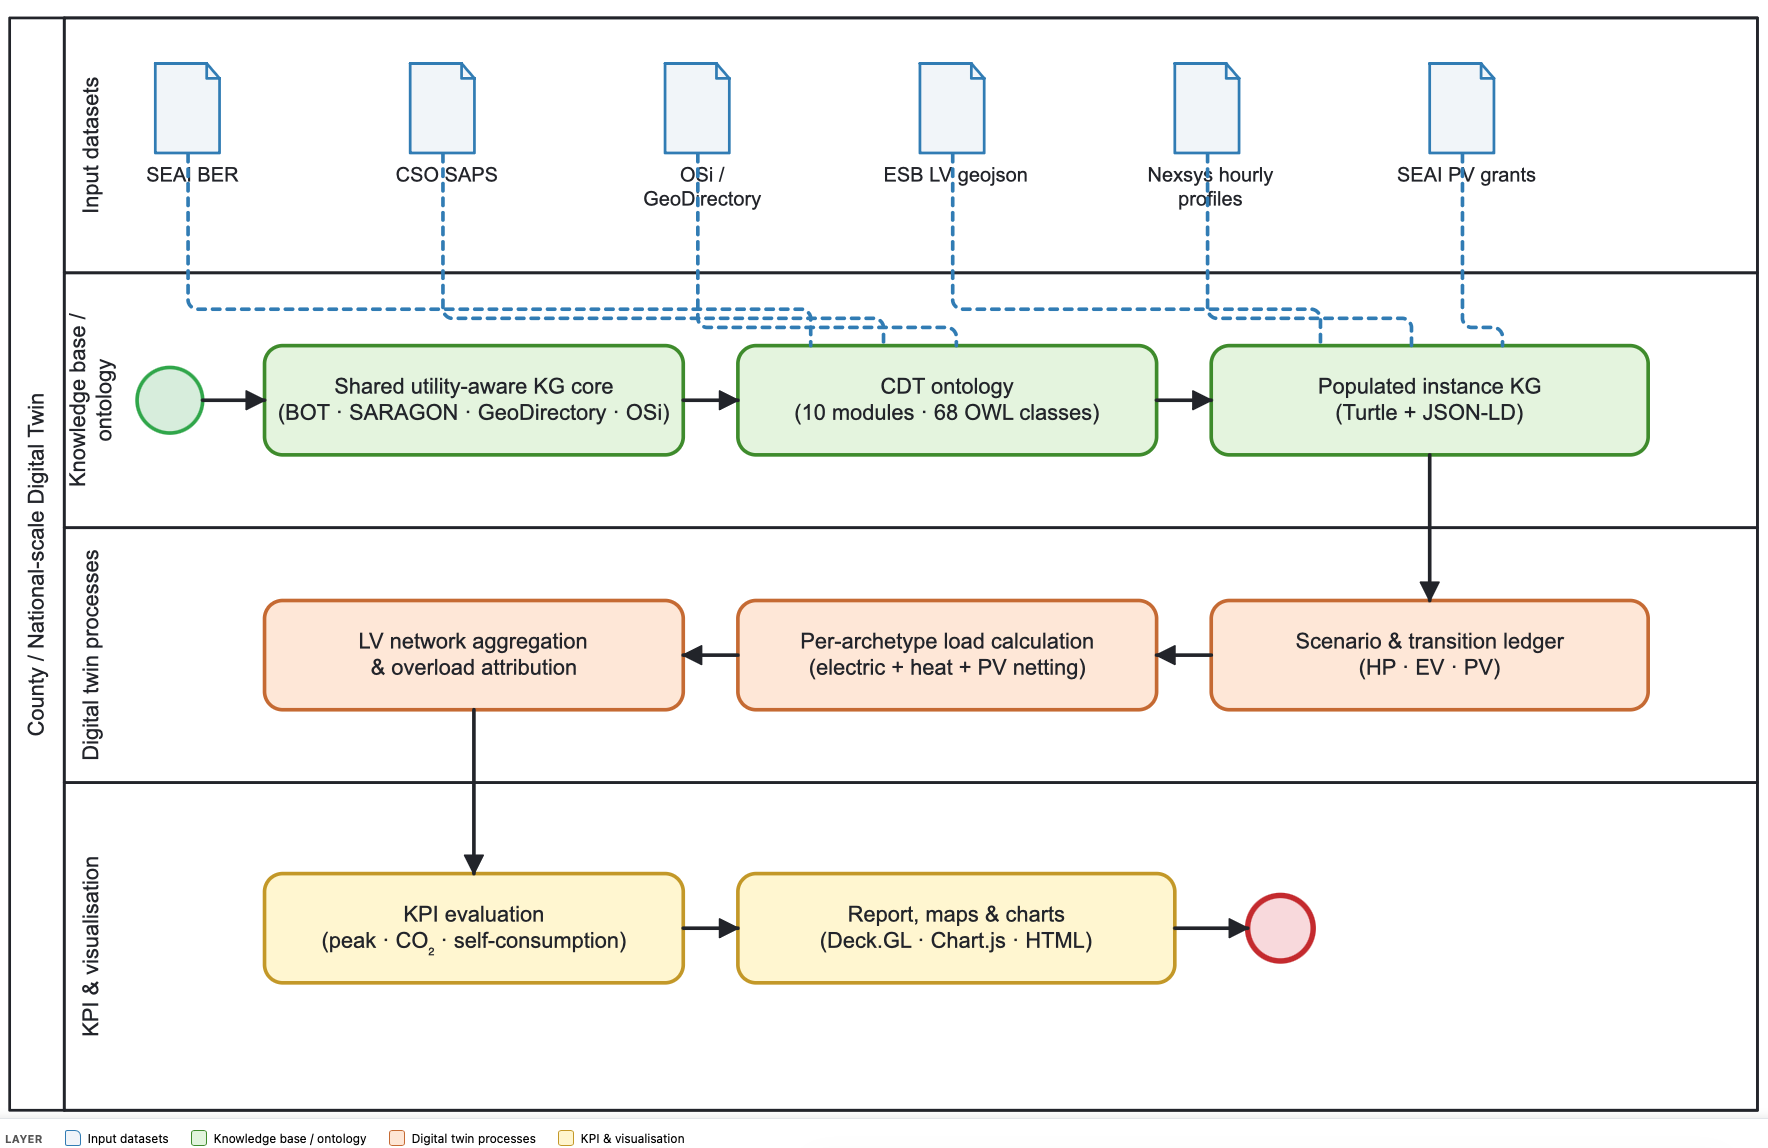
\includegraphics[width=\textwidth]{overarching.png}
  \caption{Overarching NEDT methodology. Grey elements show source datasets
    and competency questions elicited from stakeholders. Orange elements
    show the main contributions: the NEDT ontology extension, SHACL
    validation layer, and PROV-O-traceable KPI layer.}
  \label{fig:pipeline}
\end{figure}

\subsection{Implementation Architecture}
\label{sec:architecture}

The NEDT uses a two-layer pipeline.
The \emph{semantic layer} contains the OWL~2~DL T-Box ontology,
SHACL validation shapes, and an Apache Jena Fuseki SPARQL~1.1 triplestore.
This layer defines the schema, specifies competency questions as SPARQL
query patterns, constrains A-Box instances before the workflow releases
results, and records provenance through PROV-O activities.
The \emph{computational layer} uses a pandas and GeoPandas pipeline
operating on CSV and GeoJSON serialisations of the A-Box.
This layer executes demand aggregation, scenario transitions, utilisation
calculations, and cross-scale roll-up operations.

The two-layer design separates schema complexity from execution performance.
The semantic layer acts as the authoritative layer for schema validation and
competency-question specification.
The computational layer provides the execution engine for numerical planning
outputs.
Key derived outputs, including demand profiles, utilisation KPIs and
capacity flags, are written back into the triplestore as populated instance
triples so that they become queryable through SPARQL. The released Scenario~1
result graph materialises one \texttt{nedt:CapacityKPI} per evaluated LV
station and links each KPI to its station, scenario and generating PROV-O
activity. Section~\ref{sec:results:performance} reports the corresponding
SHACL validation and executed competency-question outputs.


The NEDT T-Box is not tied to a single graph store backend. The current
implementation stores the graph in Apache Jena Fuseki with SPARQL~1.1,
which was selected to support native SHACL validation and
standards-compliant SPARQL execution for competency-question evaluation.
The same OWL~2~DL T-Box can alternatively be deployed using the Neo4j
and NeoSemantic combination already demonstrated in related DDIM
work~\cite{hoare_linked_2022}, in which NeoSemantic ingests OWL and RDFS
vocabularies and maps classes, properties, and individuals to Neo4j
nodes, relationships, and labels. That deployment has been applied at
national scale in Ireland, linking the residential building stock to
over 46{,}000~LV transformers~\cite{hoare_linked_2022}, and offers a larger
developer community, simpler Cypher query syntax, and native LLM and RAG
integration suited to operational DSO environments. Every relationship in
the Neo4j property graph maps 1:1 to an RDF triple: for example,
\texttt{(b:Building)-[:NEAREST\_LV\_STATION]->(lv:LVStation)} is the
Cypher form of \texttt{nedt:isServedBy ex:b ex:lv}, so the semantic
content is identical across both backends and queries can be ported
between Cypher and SPARQL without loss of meaning. Adopters may
therefore select whichever backend fits their infrastructure without
modifying the T-Box or SHACL shape graph.


\subsection{Data Sources}
\label{sec:data-sources}

Six national datasets provide the main A-Box inputs.
Table~\ref{tab:data_sources} summarises their roles and principal
limitations.

\begin{table}[H]
\centering
\caption{Primary data sources used in the NEDT workflow.}
\label{tab:data_sources}
\small
\setlength{\tabcolsep}{4pt}
\renewcommand{\arraystretch}{1.2}
\begin{tabularx}{\textwidth}{P{3.2cm}YY}
\toprule
\textbf{Dataset} & \textbf{Role in NEDT} & \textbf{Main limitation} \\
\midrule
GeoDirectory GeoAddress and BuildingIntelligence &
  Provides the national address spine, geocoded dwelling centroids, and
  building attributes used for LV assignment. &
  Reports floor area in coarse bands; estimates construction period rather
  than surveying it directly. \\
SEAI BER Research Tool &
  Provides dwelling energy-performance attributes, heating system type, and
  archetype classification inputs. &
  Covers approximately 60\% of the national stock and is biased toward
  recently sold or retrofitted dwellings. \\
CSO Small Area Population Statistics &
  Provides Small Area dwelling counts, household structure, occupancy, and
  heating-fuel distributions for stock expansion and calibration. &
  Releases data at aggregate Small Area level; does not provide individual
  dwelling attributes. \\
ESB Networks capacity and network data &
  Provides LV station locations, capacity information, and parent-network
  relationships used for utilisation analysis. &
  May not fully expose derating, operational switching states, or exact
  nameplate values for all assets. \\
OSi administrative boundaries &
  Provides county, local authority, and Small Area geometries for spatial
  containment and hierarchical aggregation. &
  Administrative geographies do not necessarily align with electrical
  catchment boundaries. \\
CSO measured-energy series &
  Provides independent county-level electricity consumption used as a
  calibration and validation signal for aggregate demand. &
  Is too aggregated to validate individual transformer loads directly. \\
\bottomrule
\end{tabularx}
\end{table}

\subsection{Ontology Design and Semantic Scope}
\label{sec:ontology-development}

The NEDT specifies the ontology as an OWL~2~DL T-Box using a reuse-first
strategy. The released artefact includes syntax parsing, graph construction,
and SHACL-validation tests. The T-Box uses subsumption, domain and range axioms, property
inverses, one functional property and one transitive property; it does not
require the more expressive OWL~2 constructs, so the DL classification
reflects the profile it validates against rather than a claim of high
expressivity.
The ontology adopts existing vocabularies where they provide stable domain
coverage: BOT for building topology, SAREF and SAREF4ENER for device and
energy concepts, SARAGON for electricity-network assets, GeoSPARQL for
spatial representation, QUDT for quantities and units, OWL-Time for temporal
concepts, SOSA/SSN for observations, and PROV-O for provenance.

The NEDT extension introduces the classes and properties required to connect
residential building-stock modelling with distribution-network planning.
Core NEDT classes include \texttt{nedt:Archetype},
\texttt{nedt:ArchetypeCount}, \texttt{nedt:DemandProfile},
\texttt{nedt:Scenario}, \texttt{nedt:ScenarioOperator},
\texttt{nedt:TechnologyTransition}, \texttt{nedt:LVStation}, and
\texttt{nedt:CapacityKPI}.
The key connecting relationship is \texttt{nedt:isServedBy}
(domain: \texttt{nedt:Dwelling}; range: \texttt{nedt:LVStation}), which
links each dwelling to its candidate supplying transformer.
Roll-up across the network hierarchy is expressed through a transitive
super-property. \texttt{nedt:hasParentMVFeeder} and
\texttt{nedt:hasParentHVSubstation} are both sub-properties of the transitive
\texttt{nedt:hasUpstreamAsset}, whose inverse \texttt{nedt:feeds} is aligned
in intent with the SARAGON \texttt{feeds} relation. An OWL~2 reasoner
therefore entails the full $\mathsf{LV} \to \mathsf{MV} \to \mathsf{HV}$
closure from the two published one-step links, so demand can be aggregated at
any tier without materialising the closure in the A-Box. This provides a
machine-interpretable network-hierarchy pattern for downstream reasoning and
roll-up queries. The released HermiT regression test loads the T-Box,
checks that no class is unsatisfiable, and verifies the inferred two-step
LV--MV--HV relation from a minimal three-asset fixture. This test establishes
the semantic mechanism; it is not a claim that the current case-study data
has complete or verified connectivity.

The ontology aligns external vocabularies using \texttt{rdfs:subClassOf},
SKOS mapping relations, and \texttt{rdfs:seeAlso}.
At instance level the released graph contains no \texttt{owl:sameAs}
assertions. Identity across the source datasets is resolved deterministically
during extraction, on normalised station names and address identifiers, and a
single harmonised IRI is minted for the resolved entity, so no cross-graph
co-reference statement is required. We note this because
\texttt{owl:sameAs} is often assumed in linked-data integration
architectures; here the resolution happens before RDF materialisation rather
than being expressed in the graph.
Appendices~\ref{app:class-inventory} and~\ref{app:property-inventory}
provide the full class and property inventories.


\begin{figure}[H]
  \centering
  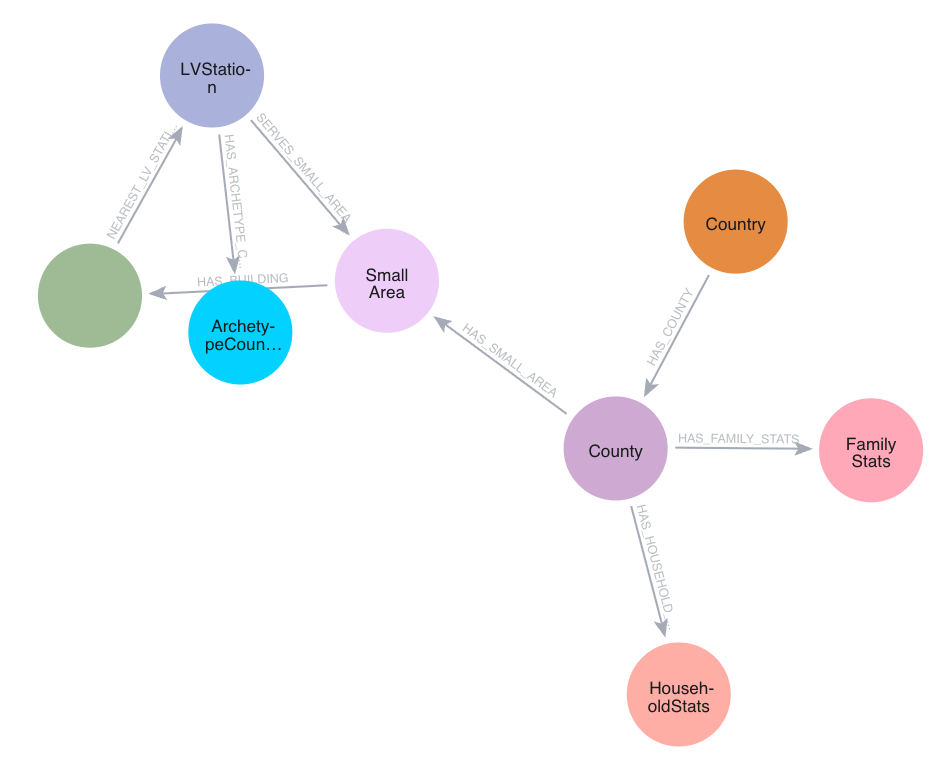
\includegraphics[width=0.8\linewidth]{Query1.png}
  \caption{Neo4j schema of the NEDT knowledge graph showing eight node
  labels (\texttt{Country}, \texttt{County}, \texttt{SmallArea},
  \texttt{Building}, \texttt{LVStation}, \texttt{ArchetypeCounts},
  \texttt{FamilyStats}, \texttt{HouseholdStats}) and eight relationship
  types. Every relationship maps 1:1 to an RDF triple --- for example,
  \texttt{(b:Building)-[:NEAREST\_LV\_STATION]->(lv:LVStation)}
  corresponds directly to \texttt{ex:b\ nedt:isServedBy\ ex:lv} ---
  making the graph queryable through both Cypher and SPARQL without
  schema modification.}
  \label{fig:neo4j-schema}
\end{figure}

\subsubsection{Competency Questions}

Fifteen competency questions frame the evaluation. They were formulated from
the planning concerns of DSO, TSO, SEAI, local-authority and DECC
stakeholders as encountered in project engagement and in the published
network and policy documents of those bodies; they are not the output of a
structured elicitation exercise with recorded participants and protocol, and
no such study is claimed here.
Section~\ref{sec:results:performance} reports which of the fifteen were
executed against the released A-Box.
CQ1--CQ2 assess archetype and building-stock representation.
CQ3--CQ4 assess scenario parameters and technology transitions.
CQ5--CQ7 assess LV station demand, overload, and flexibility indicators.
CQ8--CQ10 assess county, national, and network-level KPIs.
CQ11--CQ15 assess sensitivity, provenance, dwelling assignment, MV/HV
roll-up, and validation observations.
\ref{sec:sparql-skeletons} provides SPARQL skeletons for all
fifteen questions.

\subsection{Knowledge Graph Construction and Validation}
\label{sec:kg-construction}

The workflow constructs the NEDT graph by mapping cleaned source records into
RDF triples that instantiate the ontology.
The T-Box contains class definitions, property definitions, alignment axioms,
and SHACL shapes.
The A-Box contains populated instances derived from the source datasets.
The workflow retains source identifiers where possible and mints harmonised
NEDT IRIs for integrated entities.
Dataset-specific RDF mappers transform tabular data, while GeoJSON-to-RDF
transformations convert spatial data.
The workflow stores the graph in Apache Jena Fuseki through the DDIM server
and maintains the T-Box and A-Box as separate named graphs to support schema
stability and incremental updates.

The workflow applies SHACL validation before releasing any results.
The shape graph enforces required links, expected datatypes, and
controlled-vocabulary constraints.
The workflow accepts a graph state only when \texttt{pySHACL} reports
\texttt{conforms = true} against the full shape graph.
The validation covers both a Dublin county graph and the full national
Ireland graph.
Table~\ref{tab:shacl_validation} reports the results.

\begin{table}[H]
\centering
\caption{pySHACL validation results at county and national scope.
  Both scopes apply the same five node shapes and eleven property
  constraints.}
\label{tab:shacl_validation}
\small
\begin{tabular}{lrrrrrr}
\toprule
\textbf{Scope} & \textbf{Triples} & \textbf{Stations} &
\textbf{Archetypes} & \textbf{Stock nodes} &
\textbf{Violations} & \textbf{Elapsed (s)} \\
\midrule
Dublin  &   627{,}419 & 6{,}094 & 540 &  73{,}451 & 0 &  62.7 \\
Ireland & 3{,}330{,}755 & 36{,}234 & 741 & 388{,}606 & 0 & 347.0 \\
\bottomrule
\end{tabular}
\end{table}

Two qualifications are necessary for these results to be read correctly.

First, the \textbf{stock nodes} column counts
\texttt{nedt:ArchetypeCount} individuals, each representing a
(station, archetype) cohort, not individual dwellings. The A-Box
materialises 388,606 such cohort nodes covering 2,136,436 dwellings; it
does not instantiate 2.1 million \texttt{nedt:Dwelling} individuals. Queries
that enumerate stock at this scope therefore operate over cohorts, and
CQ13, which retrieves individual dwellings for a station, is not answerable
against this serialisation.

Second, the shape graph reported here was generated by the same script that
serialised the A-Box. A conformance result obtained this way tests
serialisation consistency, not data quality, and zero violations under such
a configuration carries little evidential weight. To address this, the
released shape graph has been rewritten to constrain value ranges,
controlled vocabularies and cross-field consistency rather than only the
presence of triples that the extraction always emits, and it is distributed
with a fixture of nine deliberately malformed instances together with a
self-test asserting that all nine are rejected. A shape graph that conforms
against that fixture is treated as broken. Appendix~\ref{app:shacl}
reproduces the shapes; the Artefact and Data Availability section gives
the repository.

Subject to those qualifications, the validation returned zero violations at
both scopes, confirming that every instance satisfies the required
cardinality, datatype and controlled-vocabulary constraints.
These validation results apply to the schema layer of the A-Box.
The pandas pipeline computes capacity KPI values --- utilisation ratios,
overload flags, and derived indicators --- and loads them into the graph as a
subsequent step, after which CQ5--CQ10 return populated result sets.

PROV-O is used to represent graph-construction, enrichment and simulation
activities, each recording source datasets, generated artefacts, processing
stage and timestamp. In the released Scenario~1 result graph, every
materialised 
\texttt{nedt:CapacityKPI} carries a
\texttt{prov:wasGeneratedBy} link to the executable scenario-workflow
activity; CQ12 verifies this path directly. Provenance coverage for the
legacy baseline A-Box remains partial, so provenance claims in this paper are
scoped to the released Scenario~1 KPI write-back rather than to every
historical analysis artefact.

\subsection{Building-to-LV Transformer Enrichment}
\label{sec:lv-enrichment}

The NEDT must link each dwelling to a candidate serving LV transformer.
Let $\mathcal{B}$ denote the set of dwellings, where each
$b \in \mathcal{B}$ has a geocoded centroid $\mathbf{p}_{b}$ in
EPSG:2157, and let $\mathcal{T}$ denote the set of LV transformers,
where each $t \in \mathcal{T}$ has a location $\mathbf{p}_{t}$ and,
where available, a service-area polygon $\mathcal{A}_{t}$.
The assignment rule selects the candidate serving transformer as
\begin{equation}
  t^{\star}(b) =
  \begin{cases}
    t \in \mathcal{T} : \mathbf{p}_{b} \in \mathcal{A}_{t},
      & \text{if a service-area polygon is available,} \\[4pt]
    \displaystyle \operatorname*{arg\,min}_{t \in \mathcal{T}}
      \lVert \mathbf{p}_{b} - \mathbf{p}_{t} \rVert_{2},
      & \text{otherwise.}
  \end{cases}
  \label{eq:assign}
\end{equation}
In the implementation reported here the second branch is the one that runs.
ESB Networks does not publish per-station service-area polygons, so no
independent polygon layer is available: the catchment polygons used for
aggregation and mapping are concave or convex hulls, or
$\sqrt{\mathrm{kVA}}$-weighted Voronoi cells, constructed \emph{from} the
nearest-transformer assignment itself. Using them as an assignment rule
would therefore be circular, and they are not used for that purpose.
All dwelling-to-transformer links in this paper are nearest-transformer
assignments, and the first branch of Equation~\eqref{eq:assign} is retained
only to show how a published connectivity layer would enter the method if a
DSO released one.
The workflow stores all geometries in Irish Transverse Mercator
(EPSG:2157), whose planar distortion across the state remains below
10~ppm, so Euclidean distances provide a faithful proxy for geodesic
distances.

The workflow materialises each assignment as
$\langle b,\;\texttt{nedt:isServedBy},\;t^{\star}(b) \rangle$
and attaches a PROV-O activity that records the enrichment method, source
data snapshots, and timestamp.

\begin{figure}[H]
  \centering
  
\includegraphics[width=\textwidth]{Fig_3_Building-LV_enrichment_BPMN_8x.png}
  \caption{Building-to-LV enrichment process.
    Dwellings are linked to candidate LV transformers using published
    service-area polygons where available and nearest-transformer
    assignment otherwise.
    The PROV-O activity records the assignment method, source snapshots,
    and timestamp.}
  \label{fig:lv-enrich}
\end{figure}

The assessment evaluates assignment accuracy using two metrics.
The \emph{dwelling-level accuracy} $\alpha$ measures the fraction of
dwellings for which the assigned transformer matches a DSO-supplied
ground-truth record.
The \emph{catchment-level Jaccard similarity} $J_\tau$ measures the ratio of
the intersection to the union of the predicted and ground-truth dwelling
sets for each transformer $\tau$, averaged across transformers.
A preliminary assessment on the Dundalk (Co.~Louth) public pilot feeders
gives $\alpha \approx 0.87$; dwellings on catchment boundaries explain most
misassignments.
This figure should be treated as indicative only. It derives from a single
town on urban and peri-urban feeders, the sample size is small, and the
underlying comparison has not been released as a reproducible artefact.
The catchment-level Jaccard similarity $J_\tau$ is defined here because it
is the appropriate metric for aggregate catchment agreement, but it has not
yet been computed, and no confidence interval is available for $\alpha$.
Dundalk is also the favourable case: rural feeders follow road corridors
that diverge most from Euclidean proximity, and it is precisely the rural
oil-heated stock that dominates the heat-pump conversion cohort.
No claim of national assignment accuracy is made in this paper.
Full ground-truth validation against a national DSO connectivity sample is
the first item of future work in Section~\ref{sec:conclusions}.

\subsection{Archetype Demand Simulation and Scenario Transitions}
\label{sec:simulation}

The simulation stage assigns hourly energy demand profiles to dwellings
through archetype simulations.
The workflow classifies each archetype by dwelling type, BER
energy-performance class, occupancy category, heating-fuel type, and weather
zone.
Let $a(b)$ denote the archetype of dwelling $b$.
Each archetype has a precomputed 8760-hour electricity and heat profile
derived from building-energy simulation using EnergyPlus and decomposed into
end-uses using the occupancy-driven method of \cite{sood_quantifying_2025}.
These profiles represent typical dwelling behaviour for each archetype
class.
Section~\ref{sec:limitations} discusses variation within archetype classes.

For archetype $a$ and scenario $S$, the scenario-specific electricity demand
at hour $h$ is
\begin{equation}
  d_{a,S}(h) =
    d_{a,0}(h)
    + \phi^{\mathrm{HP}}_{a,S}\,\Delta d^{\mathrm{HP}}_{a}(h)
    + \phi^{\mathrm{EV}}_{a,S}\,\Delta d^{\mathrm{EV}}_{a}(h)
    - \phi^{\mathrm{PV}}_{a,S}\,d^{\mathrm{PV}}_{a}(h),
  \label{eq:uplift}
\end{equation}
where $d_{a,0}(h)$ is the baseline electricity profile,
$\Delta d^{\mathrm{HP}}_{a}(h)$ is the additional electric load associated
with heat-pump conversion,
$\Delta d^{\mathrm{EV}}_{a}(h)$ is the EV charging profile, and
$d^{\mathrm{PV}}_{a}(h)$ is the rooftop PV generation.
The terms $\phi^{\mathrm{HP}}_{a,S}$, $\phi^{\mathrm{EV}}_{a,S}$, and
$\phi^{\mathrm{PV}}_{a,S}$ represent scenario adoption fractions.
The graph stores these fractions explicitly and links them to resulting
demand profiles via \texttt{nedt:evaluatedUnderScenario}.
Appendix~\ref{app:scenario-parameters} provides the Scenario~1
parameterisation.

\paragraph{Rooftop-PV construction and netting.}
The PV term is generated from the NEDT Nexsys uncontrolled-charging
workbook, rather than inferred from EV demand. For each valid archetype
sheet, the hourly \texttt{PV generation} series is divided by its own peak;
the resulting curves are averaged, zero-padded to 8760 hours where necessary,
and multiplied by $1000/1284$ to represent a 1,000~kWh/kWp/year Irish
irradiance yield. The common normalised shape is then scaled by a 2.5~kWp
system for terraced dwellings, 3.5~kWp for semi-detached dwellings, and
4.0~kWp for detached dwellings and bungalows; apartments are excluded.
At each hour, self-consumed PV reduces electricity demand only to zero, while
the configured export component is retained as net injection. This preserves
the distinction between behind-the-meter consumption and exported generation
when the station-level series is formed.

For each transformer $t$, hourly demand is the sum of the archetype profiles
of the dwellings assigned to it,
\begin{equation}
  D_{t,S}(h) =
    \sum_{a \in \mathcal{A}_t} n_{a,t}\, d_{a,S}(h),
  \label{eq:station_demand}
\end{equation}
where $n_{a,t}$ is the number of dwellings of archetype $a$ in catchment $t$,
and the coincident peak is
\begin{equation}
  P_{t,S} = \max_{h \in \{1,\ldots,8760\}} D_{t,S}(h).
  \label{eq:peak}
\end{equation}

Two properties of this operator matter for what follows.
First, it is \emph{allocate-then-maximise}: profiles are summed within the
catchment and the annual maximum is taken on that sum.
The alternative, taking a county-level maximum and distributing it by
dwelling count, is not equivalent, because it makes every station in a county
share one demand per dwelling and reduces station utilisation to a function
of the dwellings-per-kVA ratio.
Under Equation~\eqref{eq:station_demand} the archetype composition of each
catchment, and therefore BER class, occupancy and heating fuel, determines
station demand: the 37,287 modelled stations take 15,868 distinct values of
peak demand per dwelling, with a coefficient of variation of 0.41.

Second, no separate coincidence factor is applied.
The quantity $\max_h \sum_a n_{a,t} d_{a}(h)$ is already an after-diversity
maximum, because temporal diversity between archetypes is expressed in the
summation itself.
Multiplying it by a further after-diversity factor would discount diversity
twice.
The resulting national mean of 1.20~kW per dwelling, and 1.46~kW per dwelling
for the Dublin stock, sit close to the 1.5~kW after-diversity maximum demand
used in Irish and UK LV design practice, which provides an external check
that the diversity treatment is dimensionally correct.

Roll-up to MV and HV follows the same rule. The coincident peak of a parent
asset is the annual maximum of the summed hourly series of its children, not
the sum of their individual peaks. Across 467 MV feeders the coincident peak
is 0.988 of the sum of child LV peaks (IQR 0.953--0.995), so inter-catchment
diversity is real but modest at this voltage level. All voltage tiers in
Section~\ref{sec:result} derive from the same station-level series, so
utilisation values are comparable across tiers.

\subsubsection{Archetype profile coverage}
\label{sec:coverage}

The archetype-count file distinguishes 744 archetype signatures, while the
simulated profile library holds 300, structured as five dwelling types
$\times$ three heating systems $\times$ BER class $\times$ occupancy
categories 1--6. Heat-pump archetypes exist only at BER~A--B and
fossil-fuelled archetypes only at BER~B--E.
Signatures without an exact profile are served by the nearest available
profile in the same dwelling-type and heating-system cell, minimising
distance in BER and then occupancy.
Under this rule 75.7\% of dwellings match an archetype exactly and 24.3\% are
served by a neighbour.
Electrically heated dwellings (139,368) and the 98 solar-thermal dwellings
have no corresponding profile and are mapped to the heat-pump and gas
archetypes respectively.
These substitutions are recorded per record and are a limitation of the
profile library rather than of the method; Section~\ref{sec:limitations}
discusses their effect.

\subsubsection{Demand validation}
\label{sec:calibration}

Aggregating the station-level series of Equation~\eqref{eq:station_demand} to
county level gives an independent check against CSO metered residential
electricity consumption for 2024.
No calibration factor is applied: the comparison is between raw simulated
demand and measured consumption.
Table~\ref{tab:county_validation} reports the result.
Modelled national consumption is 8,477~GWh against 8,943~GWh metered, a
normalised mean bias error of $-5.2\%$, with a mean absolute percentage error
of 11.8\% and a CV(RMSE) of 11.2\% across the 26 counties, and a coefficient
of determination of 0.9935.
These are descriptive errors over 26 annual spatial aggregates. They are
not monthly time-series calibration statistics and must not be compared with
ASHRAE Guideline~14 monthly-calibration thresholds. The comparison therefore
checks only approximate aggregate-volume consistency; it does not validate
hourly peaks, transformer assignment, or capacity classifications.

This replaces the county calibration used in earlier versions of this
workflow, in which modelled electricity was multiplied by county-specific
factors ranging from 0.745 to 1.444 so that totals reconciled with CSO.
Those factors are not used here.
The residual county errors reported in
Table~\ref{tab:county_validation} range from $-19.8\%$ to $+23.6\%$ and are
largest in counties with sparse BER coverage, which indicates that the
remaining error is a property of the stock characterisation rather than of
the demand operator.

\begin{table}[H]
\centering
\caption{County-level validation of modelled residential electricity against
  CSO metered consumption, 2024. No calibration factor is applied.}
\label{tab:county_validation}
\small
\begin{tabular}{lrrr}
\toprule
\textbf{Indicator} & \textbf{Value} & \textbf{Interpretation} & \textbf{Met} \\
\midrule
Counties compared            & 26        & ---            & --- \\
Modelled national total      & 8{,}477~GWh & ---          & --- \\
Metered national total (CSO) & 8{,}943~GWh & ---          & --- \\
NMBE                         & $-5.2\%$  & annual aggregate error & --- \\
MAPE                         & 11.8\%    & ---            & --- \\
CV(RMSE)                     & 11.2\%    & annual aggregate error & --- \\
$R^{2}$                      & 0.9935    & dominated by county size & --- \\
\midrule
Largest positive error       & Donegal, $+23.6\%$ & --- & --- \\
Largest negative error       & Monaghan, $-19.8\%$ & --- & --- \\
\bottomrule
\end{tabular}
\smallskip
\noindent\footnotesize{No ASHRAE compliance claim is made: these are annual
county totals, not monthly calibration observations.}
\end{table}

\subsection{Capacity and Overload Indicators}
\label{sec:overload}

The following indicator is a \emph{screening proxy}, not a transformer
thermal-loading measurement. It becomes an engineering loading assessment
only when real and reactive power, temperature/derating, switching state,
and a validated service connection are available. Consequently, threshold
counts in this paper identify candidates for DSO study rather than verified
overloads.

Given the coincident peak demand $P_{t,S}$ from
Equation~\eqref{eq:peak}, the workflow calculates transformer utilisation as
\begin{equation}
  U_{t,S} =
    \frac{P_{t,S} / \mathrm{pf}}{C_t \, k_{\theta}},
  \label{eq:utilisation}
\end{equation}
where $C_t$ is the rated capacity from the ESB Networks asset register,
$\mathrm{pf}$ is an effective load power factor converting real power to
apparent power, and $k_{\theta} = 1 + 0.005\,(\theta_{\mathrm{rated}} -
\theta_{\mathrm{amb}})$ is the IEC~60076-2 ambient correction, clamped to
$[0.85, 1.20]$.
The implementation computes $\mathrm{pf}$ as a load-weighted mean
($\mathrm{pf} = 0.95$ base, $0.87$ heat pump, $0.97$ EV).
\textbf{For the results reported in Section~\ref{sec:result}, both
corrections are inactive ($\mathrm{pf} = 1$, $k_{\theta} = 1$), so
utilisation is computed as real power in kW divided by rated apparent power
in kVA.} Because a transformer thermal rating is a kVA constraint, this
understates utilisation by a factor of $1/\mathrm{pf}$, approximately 5\% at
baseline and more under heat-pump uptake, where inverter drives lower the
effective power factor. We state this explicitly rather than leave it
implicit in the units.

The workflow classifies a transformer as \emph{over-capacity} when
$U_{t,S} > 1.0$ and as \emph{near-capacity} when
$0.9 \leq U_{t,S} \leq 1.0$.
For MV and HV assets, the workflow aggregates LV-level demands through the
parent-feeder hierarchy.

\paragraph{Capacity imputation}
Rated capacity is unavailable for 954 of the 37,287 stations
(2.6\%). These stations are assigned a default of 200~kVA.
Only 16 of the 3,009 over-capacity stations (0.5\%) carry an imputed rating,
so the headline counts are not materially driven by the substitution.
Because the denominator of Equation~\eqref{eq:utilisation} is the rated
capacity, an imputed rating determines over-capacity status
deterministically for the affected assets, whatever their modelled demand.
Individual station verdicts for imputed assets are not evidence, but the
national totals are insensitive to the choice.
The graph flags these stations with \texttt{nedt:hasCapacityImputed}, and
the SHACL shape graph requires the flag on every station, so that imputed
capacities cannot propagate silently into KPIs.
Utilisation estimates additionally carry interval uncertainty where the
published capacity is banded rather than exact, so comparisons close to the
100\% threshold should be interpreted with caution.


%%=========================================================================
\section{Results}
\label{sec:result}
%%=========================================================================

This section reports four sets of results: knowledge graph coverage and
enrichment quality; the 2024 baseline capacity status across LV, MV, and
HV tiers; scenario impacts under a compound residential electrification
case; and SHACL-conformant competency-question evaluation against the
populated national result graph.

\subsection{Knowledge Graph Coverage and Enrichment}
\label{sec:results:kg}

The constructed knowledge graph contains \textbf{2,137,827 nodes} across
four entity types: 26 counties, 13,254 Small Areas, 46,377 LV substations,
and 2,078,170 georeferenced residential building records.
Building and dwelling counts differ throughout this paper and are not
interchangeable: a building record may contain more than one dwelling, so the
2,078,170 building records correspond to the 2,136,436 dwellings carried
through the demand analysis.
Approximately \textbf{4.20 million directed edges} encode
building-to-Small-Area containment (2,078,170), building-to-LV-station
assignment (2,078,170), and station-to-county location links (46,377).
Of the 46,377 substations in the graph, 41,309 match at least one
residential building.
The remaining substations likely serve non-residential or sparsely populated
areas.

Three station populations appear in this paper and are not
interchangeable. The spatial graph contains 46,377 substations, of which
41,309 have at least one assigned building. The capacity analysis in
Sections~\ref{sec:results:baseline} and~\ref{sec:results:scenario} covers
the 37,287 stations that carry a BER-matched archetype demand profile.
The serialised A-Box used for SHACL validation and
competency-question benchmarking
(Sections~\ref{sec:kg-construction} and~\ref{sec:results:performance})
contains 36,234 stations, being the 37,287 less 1,053 whose county could
not be resolved and which were therefore excluded from the RDF export.

The building-to-transformer assignment has a median distance of
\textbf{134.6~m} and a mean distance of \textbf{435.7~m}.
The enrichment process assigns 65.2\% of buildings within 200~m, 85.5\%
within 1~km, and 95.4\% within 2~km.
A small tail of 3,068 buildings, equivalent to 0.15\%, have assignment
distances above 5~km, concentrated in sparse western rural areas.
Urban counties show shorter assignment distances, while rural western
counties show longer distances, consistent with lower transformer density in
those regions.
These distance statistics describe spatial proximity; they do not directly
measure assignment accuracy.
The preliminary dwelling-level accuracy from the Dundalk pilot
($\alpha \approx 0.87$) gives the best available accuracy estimate.
Future work will complete full national ground-truth validation.

\subsection{Baseline Network Capacity}
\label{sec:results:baseline}

The 2024 baseline represents as-is residential demand before the workflow
applies any additional HP, EV, or rooftop PV adoption.
National hourly electricity demand shows little seasonal trend, though it
cycles daily between roughly 0.2 and 2.8~GWh/h, while heat demand is
strongly seasonal with winter peaks near 9~GWh/h.

\begin{figure}[H]
  \centering
  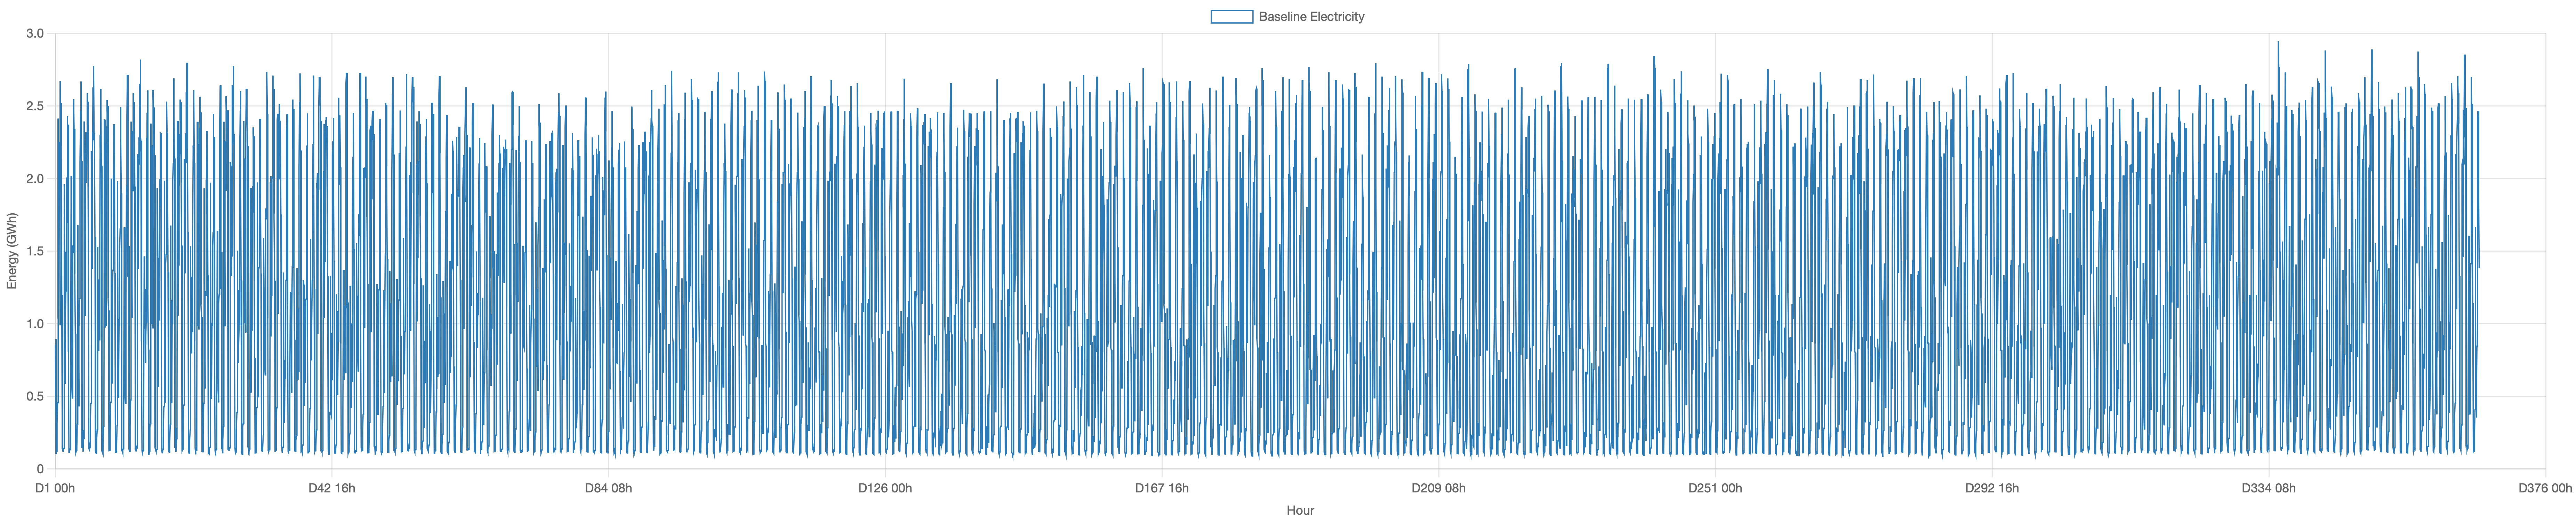
\includegraphics[width=\linewidth]{asis_2024_electricity.png}\\[4pt]
  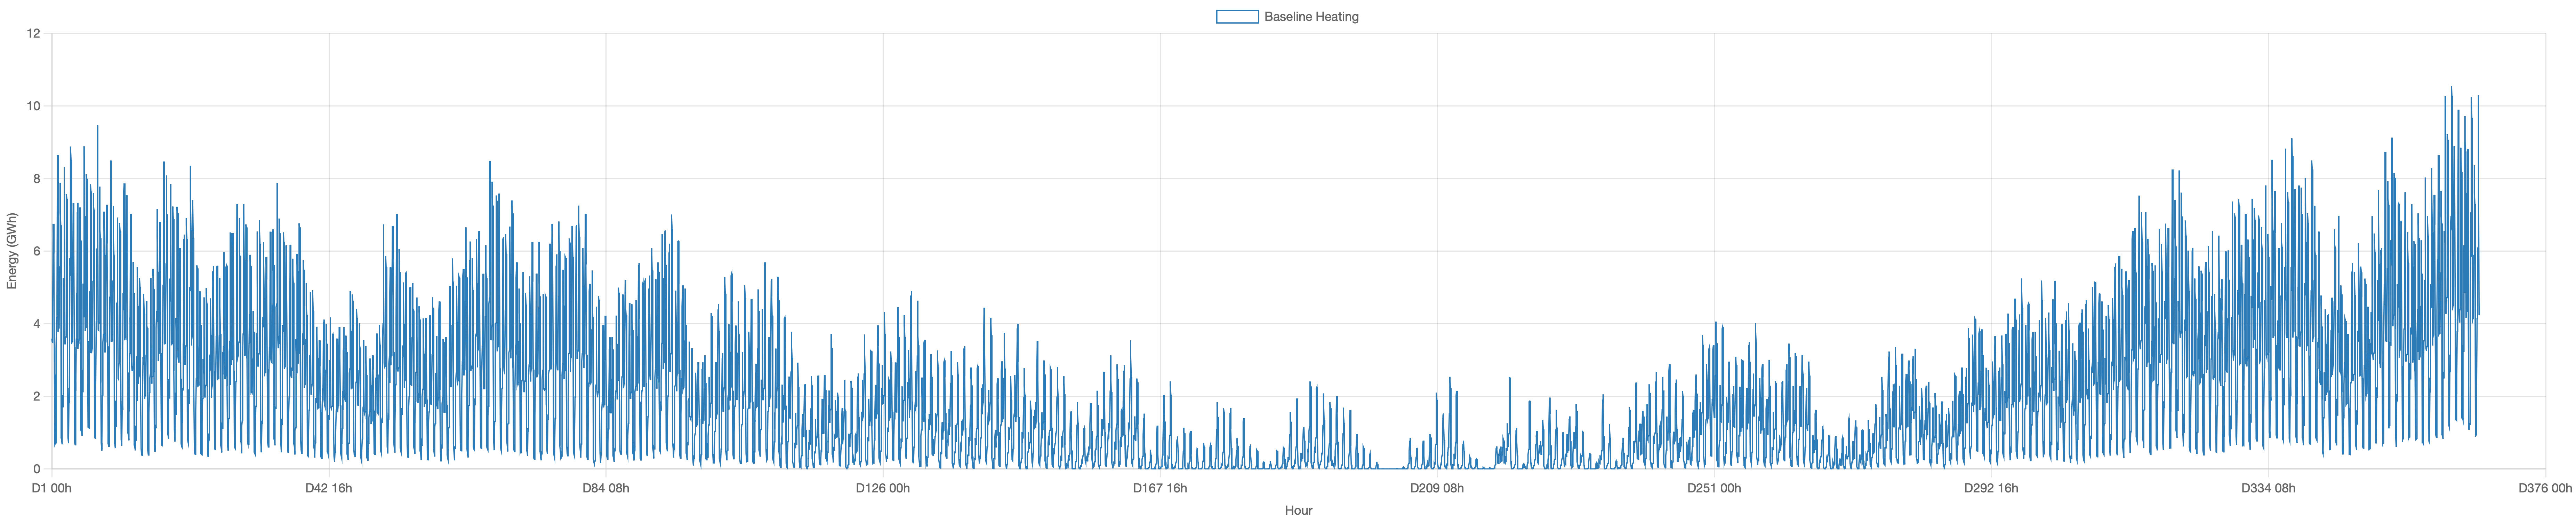
\includegraphics[width=\linewidth]{asis_2024_fossil.png}\\[4pt]
  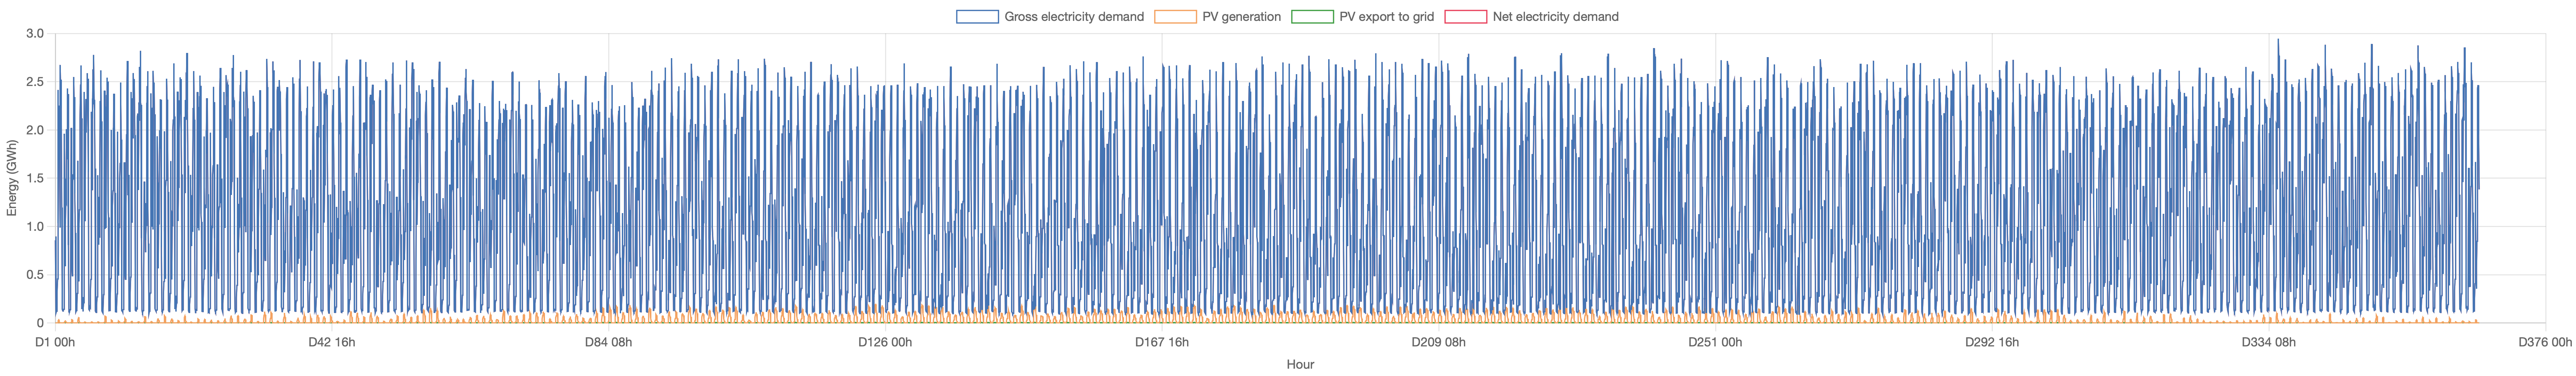
\includegraphics[width=\linewidth]{asis_2024_pv.png}
  \caption{Baseline 2024 national hourly profiles.
    \textit{Top}: electricity demand.
    \textit{Middle}: aggregated fossil heat demand.
    \textit{Bottom}: rooftop PV generation.}
  \label{fig:baseline_ts}
\end{figure}

The baseline model covers 37,287 MV/LV substation catchments with
BER-matched residential demand profiles and serves 2,136,436 dwellings.
These LV catchments roll up to 496 MV feeders and 100 HV substations
(Table~\ref{tab:baseline_network_scope}).

\begin{table}[H]
\centering
\caption{Network scope of the 2024 baseline by voltage tier.}
\label{tab:baseline_network_scope}
\small
\begin{tabular}{lrrl}
\toprule
\textbf{Voltage tier} & \textbf{Assets modelled} &
  \textbf{Dwellings served} & \textbf{Source} \\
\midrule
LV, MV/LV substations & 37{,}287 & 2{,}136{,}436 &
  ESB Networks + BER archetype file \\
MV, 38\,kV feeders    &    496   & --             &
  ESB parent linkage \\
HV, 110/220\,kV nodes &    100   & --             &
  Upstream nodes with TSO interface \\
\bottomrule
\end{tabular}
\end{table}

Table~\ref{tab:breach_summary} summarises baseline utilisation across
all three voltage tiers.
At LV level, 3,009 stations, or 8.1\%, already exceed rated capacity and
serve 304,878 dwellings.
A further 609 LV stations fall in the 90--100\% near-capacity band.
At MV level, 4 of 467 feeders exceed rated capacity.

Peak demand per dwelling is no longer uniform across the estate. It has a
national mean of 1.20~kW and a median of 1.227~kW, with a 5th--95th
percentile range of 0.671--1.820~kW and 15,868 distinct values. It also rises
systematically with transformer size, from a mean of 1.03~kW per dwelling on
units rated at or below 50~kVA to 1.47~kW on units above 400~kVA, reflecting
the larger and less efficient dwellings typically served by larger
transformers. Dublin, with its higher apartment and gas-heating share, has a
mean of 1.46~kW per dwelling against the national 1.20~kW.
All HV substations remain below 90\% utilisation.

\begin{table}[H]
\centering
\caption{As-is 2024 capacity status by voltage tier.
  \textit{Near-capacity} = 90--100\% utilisation.
  All tiers derive from the same station-level hourly series of
  Equation~\eqref{eq:station_demand}; MV and HV values are coincident
  roll-ups, not independently parameterised runs. The Dublin row is the
  subset of stations in that county, shown because the archetype mix there
  differs markedly from the national stock.}
\label{tab:breach_summary}
\small
\begin{tabularx}{\textwidth}{Xrrrrrr}
\toprule
\textbf{Voltage tier} &
\textbf{Total} & \textbf{Red $>$100\%} & \textbf{Near-cap.} &
\textbf{Stressed} & \textbf{OK} & \textbf{Peak util.} \\
\midrule
LV, national   & 37{,}287 & 3{,}009 & 609 & 9.7\% & 33{,}669 & 997\% \\
LV, Dublin area &  6{,}348 &     118 &  54 & 2.7\% &  6{,}176 & 553\% \\
MV, 38\,kV     &    467   &       4 &   2 & 1.3\% &    461   & 144\% \\
HV, 110/220\,kV &   108   &       0 &   0 & 0.0\% &    108   &  --- \\
\bottomrule
\end{tabularx}
\end{table}

The LV stress pattern varies strongly across space.
Figure~\ref{fig:lv_national} shows that urban cores --- Dublin, Cork,
Limerick, and Galway --- generally have lower stress, reflecting higher
substation density and a more recently reinforced network.
Rural and peri-urban catchments show higher concentrations of over-capacity
and near-capacity stations.
In these areas, smaller legacy transformers, predominantly 50~kVA units
installed between the 1970s and 1990s, now serve catchments whose dwelling
counts have grown substantially since the original network construction.

\begin{figure}[H]
  \centering
  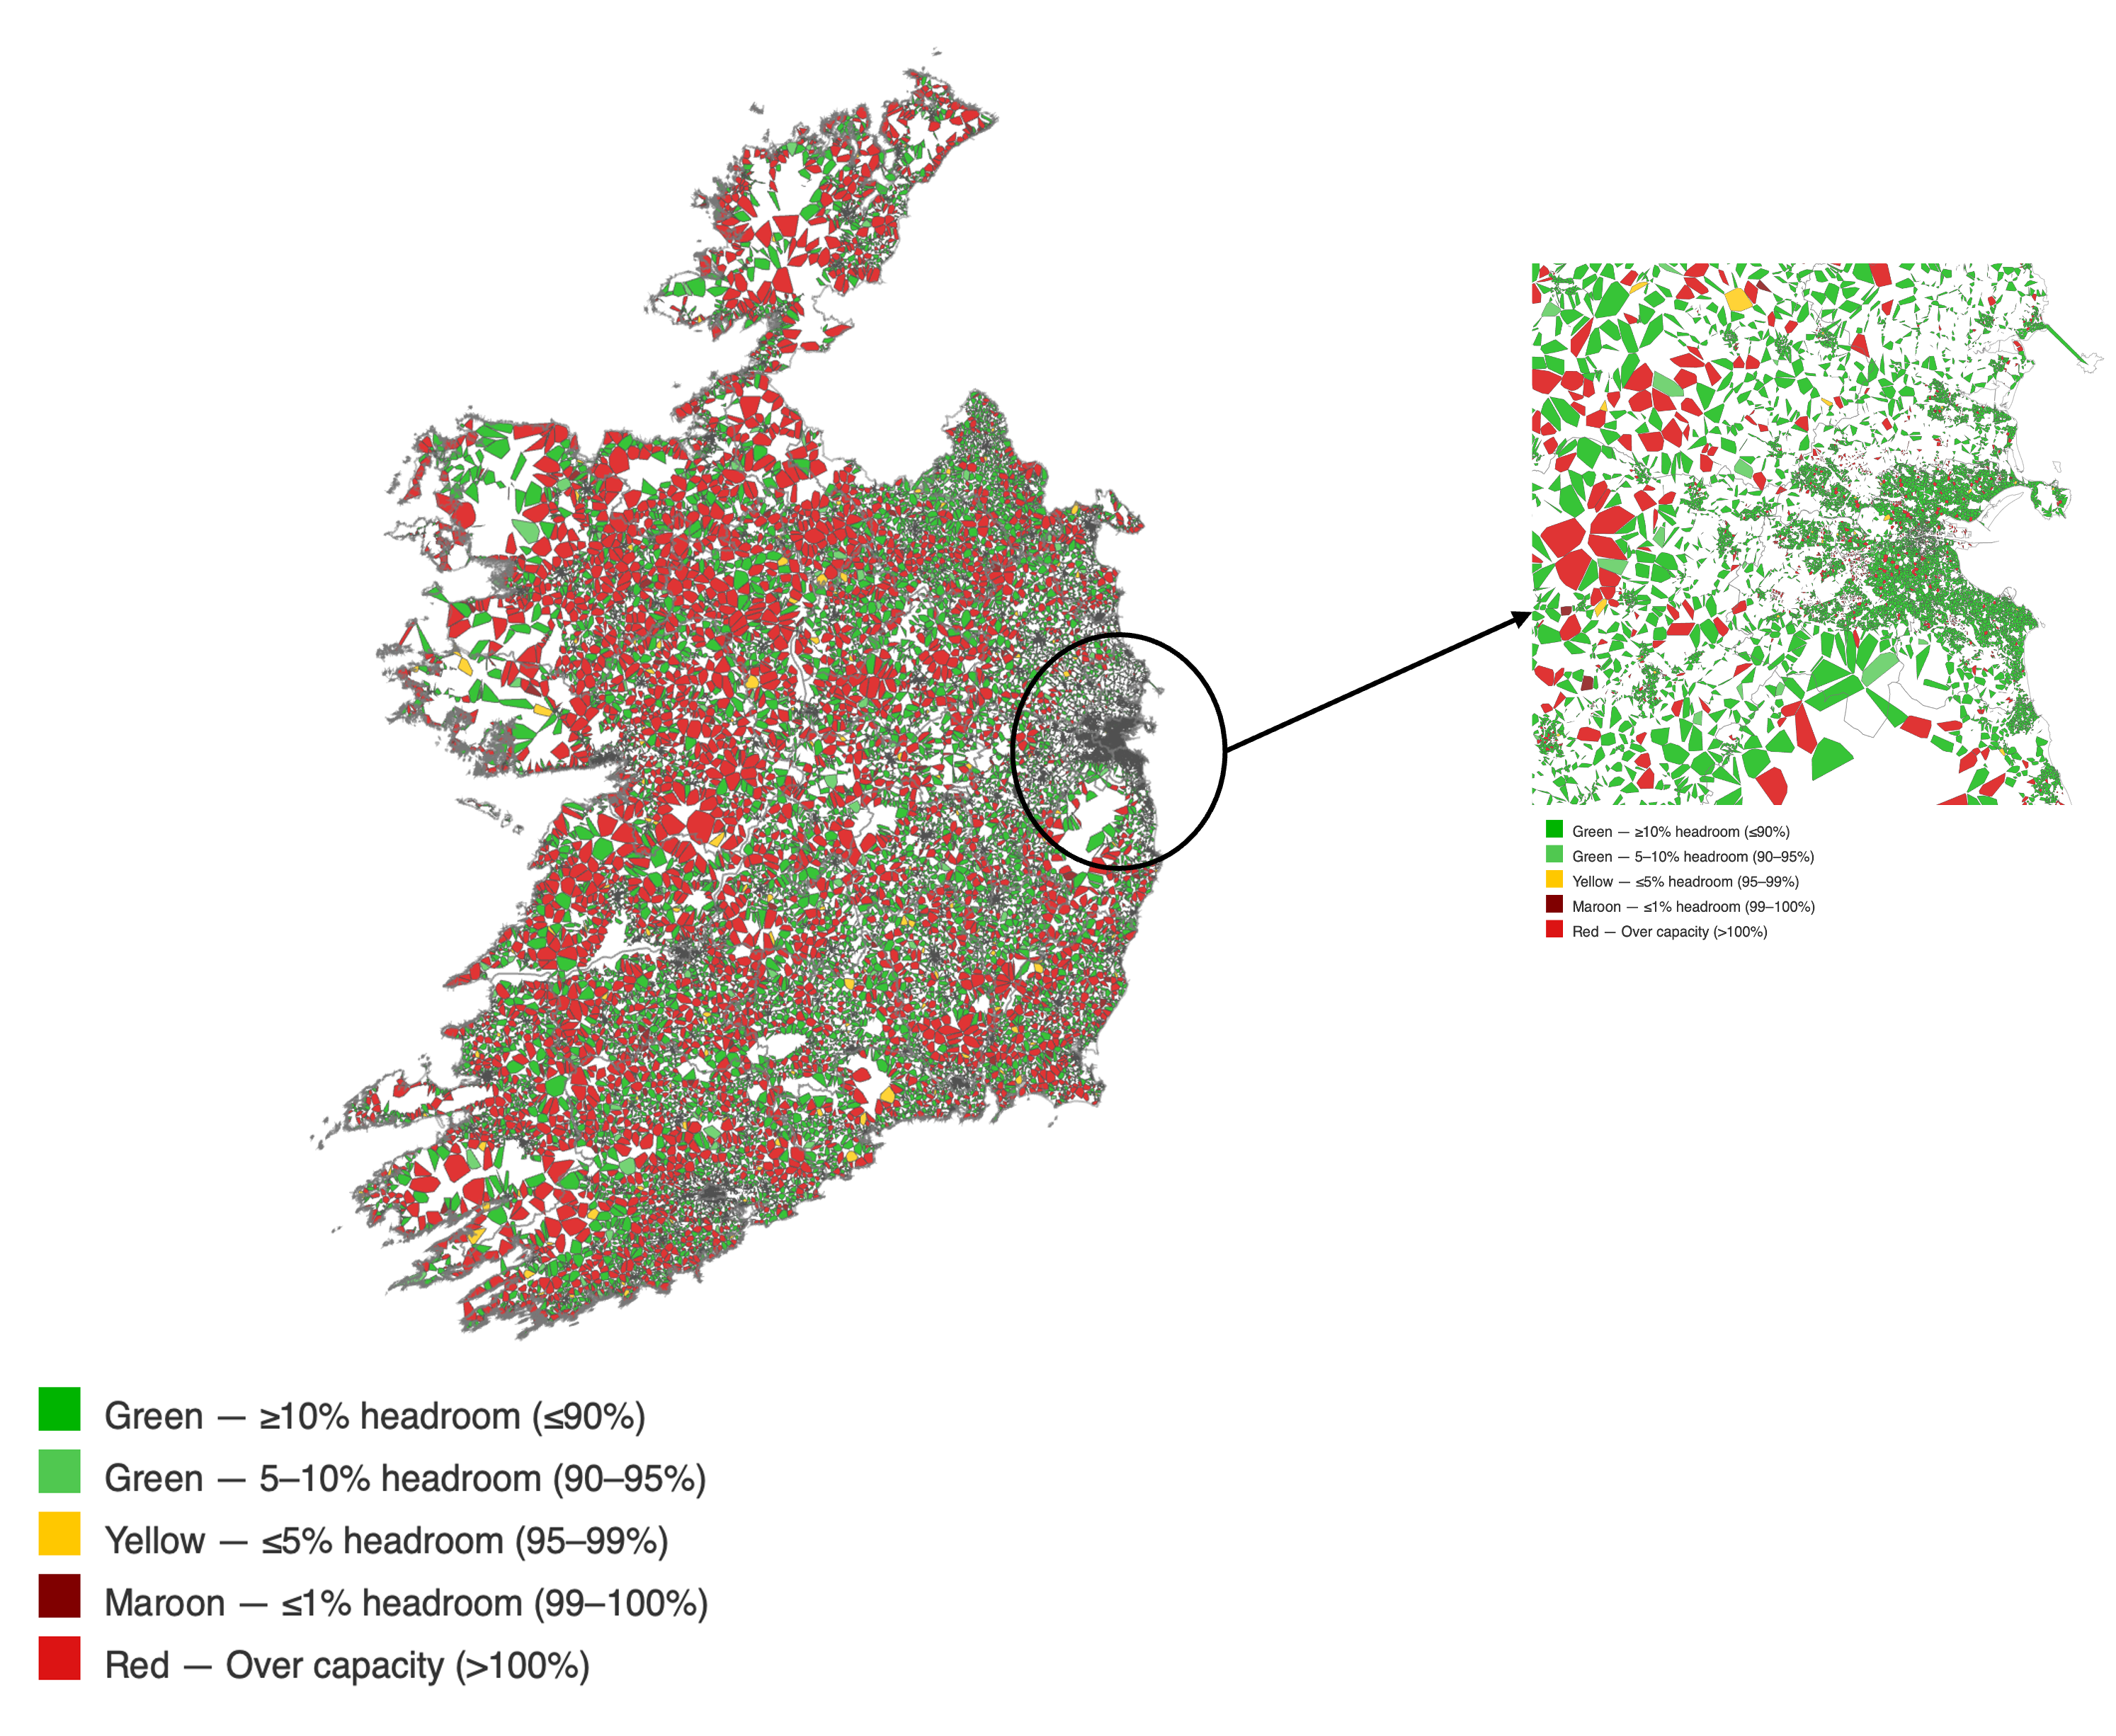
\includegraphics[width=\linewidth]{asis_2024_lv_combined.png}
  \caption{LV station utilisation under the 2024 baseline.
    Each polygon represents the Voronoi service area of one LV station,
    coloured by peak utilisation band.
    Grey outlines show county boundaries.}
  \label{fig:lv_national}
\end{figure}

Table~\ref{tab:lv_breach_ranked} ranks the highest-utilisation LV
transformers nationally.
Of the 3,009 over-capacity stations, 79.3\% have a 50~kVA rating, the
smallest standard unit in the ESB Networks plant.
These transformers were sized for loads dominated by electric lighting and
resistive appliances.
Unlike a dwellings-per-kVA screen, this ranking responds to catchment
composition: the listed stations span 1.13--1.54~kW per dwelling, so two
catchments of similar size can differ by a third in modelled peak according
to their archetype mix.
Only 16 of the 3,009 over-capacity stations carry an imputed rated capacity.

\begin{table}[H]
\centering
\caption{Ten highest-utilisation LV transformers nationally in the 2024
  baseline. Station identifiers are anonymised per data-sharing protocol.
  Excess power is peak demand minus rated capacity. No station in this
  ranking has an imputed rated capacity.}
\label{tab:lv_breach_ranked}
\small
\begin{tabular}{lrrrrc}
\toprule
\textbf{Station} & \textbf{Bldgs} & \textbf{Rated (kVA)} &
  \textbf{kW/dwell.} & \textbf{Util.\ (\%)} & \textbf{Excess (kW)} \\
\midrule
BA***166Z & 3{,}236 & 400 & 1.23 & 996.7 & +3{,}586.8 \\
KI***4037 &    295  &  50 & 1.54 & 907.5 &   +403.8 \\
TU***002X &    307  &  50 & 1.40 & 862.2 &   +381.1 \\
PR***419  &    237  &  33 & 1.15 & 826.6 &   +239.8 \\
CR***323Y &    310  &  50 & 1.23 & 763.8 &   +331.9 \\
TE***507  &    323  &  50 & 1.13 & 731.6 &   +315.8 \\
BR***4060 &    306  &  50 & 1.14 & 698.1 &   +299.1 \\
HO***265  &    273  &  50 & 1.23 & 672.4 &   +286.2 \\
DO***4103 &    267  &  50 & 1.23 & 656.6 &   +278.3 \\
FA***4180 &    568  & 100 & 1.15 & 651.0 &   +551.0 \\
\bottomrule
\end{tabular}
\end{table}

At MV level, Table~\ref{tab:mv_baseline_breach} lists the four
over-capacity 38~kV feeders under the coincident roll-up.
These differ from the feeders identified in earlier versions of this
workflow, which computed MV demand on a separate basis from LV; the values
below are the annual maximum of the summed hourly series of each feeder's
child LV stations, so they are consistent with
Table~\ref{tab:breach_summary} by construction.

\begin{table}[H]
\centering
\caption{MV (38~kV) feeders exceeding rated capacity in the 2024 baseline,
  as coincident roll-ups of the per-catchment LV series.}
\label{tab:mv_baseline_breach}
\small
\begin{tabular}{lrrr}
\toprule
\textbf{Feeder} & \textbf{Peak (kW)} & \textbf{Rated (kVA)} &
  \textbf{Util.\ (\%)} \\
\midrule
Portarlington  & \phantom{0}7{,}205 & \phantom{0}5{,}000 & 144.1 \\
Turlough Road  & \phantom{0}6{,}490 & \phantom{0}5{,}000 & 129.8 \\
Kinsale        &           11{,}680 &           10{,}000 & 116.8 \\
Buttevant      & \phantom{0}4{,}248 & \phantom{0}4{,}000 & 106.2 \\
\bottomrule
\end{tabular}
\end{table}

\subsection{Electrification Scenario Impacts}
\label{sec:results:scenario}

Scenario~1 is an illustrative planning case, designed to demonstrate how
technology-transition assumptions propagate through the NEDT information
model. It is not intended as a forecast of realised adoption or a substitute
for asset-specific network studies.

Scenario~1 represents a near-term compound adoption case that combines
heat-pump, EV, and rooftop PV uptake.
Appendix~\ref{app:scenario-parameters} provides the full parameterisation.
The scenario converts 20\% of eligible BER~C--E oil-heated and gas-heated
dwellings to heat pumps.
It sets EV penetration at 10\% of the national private-car stock and rooftop PV penetration at
10\% of eligible non-apartment dwellings.

Scenario~1 converts 20\% of eligible BER~C--E oil- and gas-heated dwellings
to heat pumps, a national total of 210,843 conversions, equips 243,265
dwellings with EV chargers, and applies rooftop PV to 183,108 eligible
non-apartment dwellings.
Of the 168,459 incremental EV assignments, 6,844 (4.1\%) are allocated to
heat-pump-transition cohorts; HP--EV co-adoption is therefore represented
explicitly rather than excluded.
Table~\ref{tab:hp_by_type} shows that detached oil-boiler dwellings form
the largest HP adoption cohort.
This reflects Ireland's rural housing stock outside the gas network.

\begin{table}[H]
\centering
\caption{Eight largest heat-pump adoption cohorts by building type and
  incumbent fuel under Scenario~1, aggregated over BER and occupancy
  classes. Smaller bungalow, duplex, temporary-structure and terraced-house
  cohorts are retained in the machine-readable transition ledger.}
\label{tab:hp_by_type}
\small
\begin{tabular}{llr}
\toprule
\textbf{Building type} & \textbf{Incumbent fuel} & \textbf{HP units} \\
\midrule
Detached     & Oil boiler  &  67{,}129 \\
SemiDetached & Gas boiler  &  46{,}023 \\
Terraced     & Gas boiler  &  33{,}089 \\
SemiDetached & Oil boiler  &  29{,}242 \\
Apartment    & Gas boiler  &  14{,}579 \\
Detached     & Gas boiler  &  10{,}573 \\
Terraced     & Oil boiler  &   8{,}487 \\
Apartment    & Oil boiler  &   1{,}644 \\
\bottomrule
\end{tabular}
\end{table}

\begin{figure}[H]
  \centering
  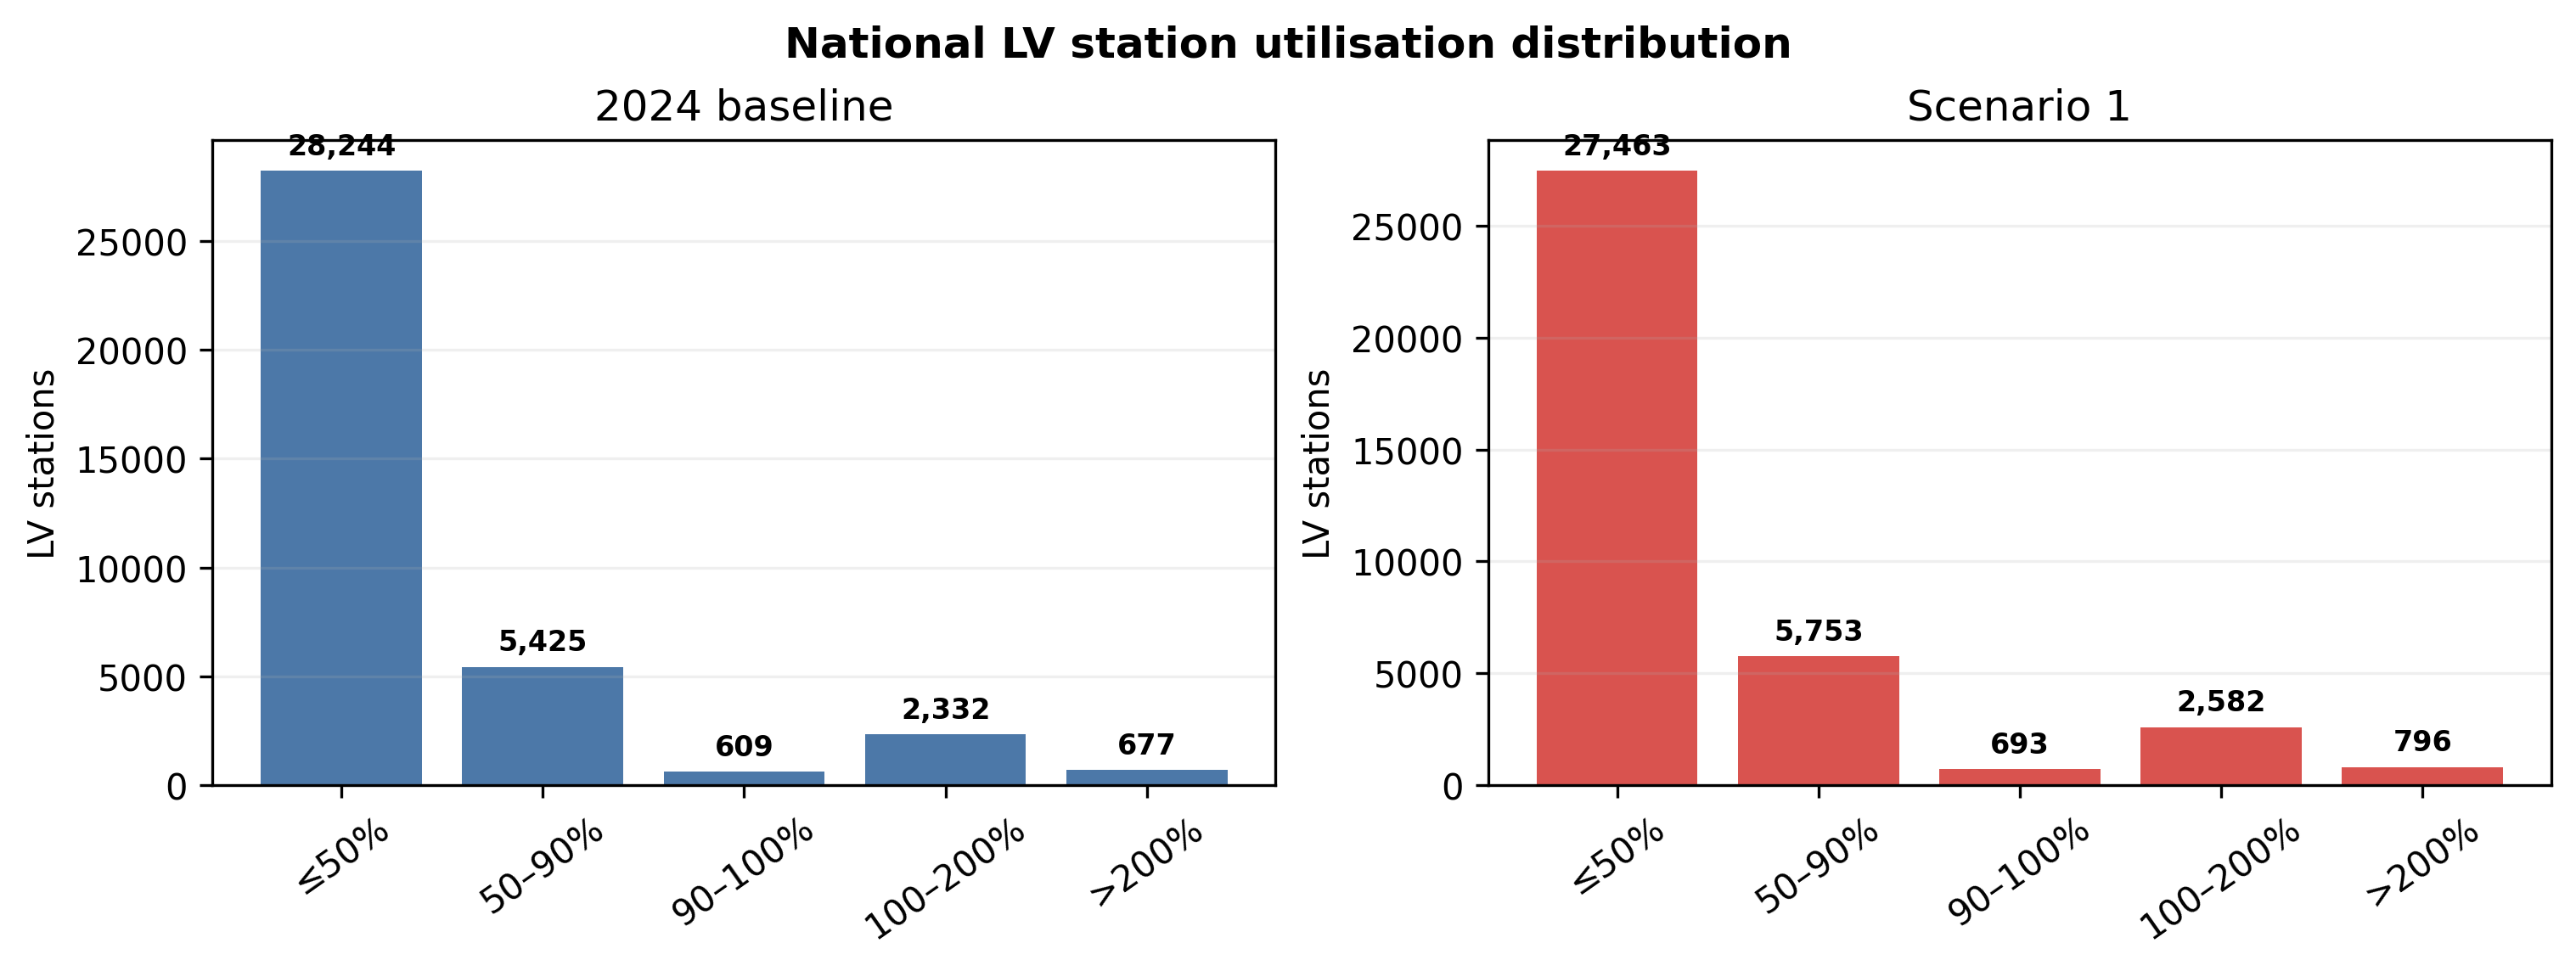
\includegraphics[width=\linewidth]{scenario1_lv_summary.png}
  \caption{National LV utilisation distribution under the regenerated
    Scenario~1 workflow (HP + EV + PV per
    Appendix~\ref{app:scenario-parameters}), compared with the 2024
    baseline.}
  \label{fig:lv_national_s1}
\end{figure}

Figure~\ref{fig:lv_national_s1} shows LV utilisation under Scenario~1.
Because baseline and scenario are computed from the same operator and the
same profile library, the two are directly comparable.
Table~\ref{tab:lv_scenario_summary} reports the national LV result.

\begin{table}[H]
\centering
\caption{National LV capacity status under Scenario~1 compared with the
  2024 baseline, both computed with Equation~\eqref{eq:station_demand}.
  \textit{Near-capacity} = 90--100\% utilisation.}
\label{tab:lv_scenario_summary}
\small
\begin{tabular}{lrrr}
\toprule
\textbf{Indicator} & \textbf{Baseline} & \textbf{Scenario~1} &
  \textbf{Change} \\
\midrule
Stations modelled                     & 37{,}287 & 37{,}287 & --- \\
Over-capacity ($>$100\%)              &  3{,}009 &  3{,}378 & $+$369 \\
Near-capacity (90--100\%)             &     609  &     693  & $+$84 \\
Stressed (\%)                         &    9.70\% &  10.92\% & $+$1.2~pp \\
Dwellings in over-capacity catchments & 304{,}878 & 343{,}973 & $+$39{,}095 \\
95th-percentile utilisation           &   128.1\% &   136.8\% & $+$8.7~pp \\
99th-percentile utilisation           &   246.2\% &   264.9\% & $+$18.7~pp \\
Mean peak per dwelling                &  1.203~kW &  1.275~kW & $+$6.0\% \\
\midrule
\multicolumn{4}{l}{\textit{Origin of the 401 newly over-capacity stations}} \\
\quad from near-capacity band (90--100\%) & --- & 245 & 61.1\% \\
\quad from below 90\% utilisation         & --- & 156 & 38.9\% \\
\bottomrule
\end{tabular}
\end{table}

\paragraph{Asset and connectivity quality screen.}
The workflow retains all stations in the national model-screened statistics,
but distinguishes a reconciliation cohort from interpretable screening
candidates. An asset enters this cohort when its modelled utilisation exceeds
500\% or its archetype input represents more than 1,000 dwellings. The screen
flags 46 stations (14,115 modelled dwellings; 1.36\% of the 3,378 red flags).
They are retained for data-quality prioritisation, not presented as routine
reinforcement candidates, and are reported separately in
Table~\ref{tab:lv_reconciliation_exceptions} and the machine-readable
\texttt{asset\_reconciliation\_exceptions.csv} artefact.

The highest modelled value, 1,154.6\%, is an input-reconciliation exception,
not a headline planning result. For BA***166Z, the archetype input assigns
3,236 dwellings whereas the independent building-to-station assignment file
contains 1,868 dwellings (a ratio of 1.73). The published availability
snapshot lists 400~kVA installed capacity and 78~kVA allocated load (19.5\%
utilisation). That snapshot is not time-aligned overload ground truth, but
the discrepancy precludes interpreting the modelled 4.62~MW peak as an
observed overload. Across the 46 records, 20 have an archetype-to-assignment
dwelling ratio outside $\pm20\%$ and 16 have an availability utilisation at
or below 20\%. The executable workflow therefore materialises this count
reconciliation diagnostic for every station. The all-station distribution is
reported with robust 95th and 99th percentiles in
Table~\ref{tab:lv_scenario_summary}; its maximum is not used to characterise
national planning exposure.

The scenario response is heterogeneous, which is the substantive difference
from a uniformly scaled projection.
The per-station ratio of scenario to baseline peak has a mean of 1.058 and a
median of 1.000, but ranges from 0.989 at the 5th percentile to 1.261 at the
95th, across 3,779 distinct values after rounding to four decimal places.
Stations therefore change rank under the scenario, and the assets that move
into the over-capacity band are those whose catchments actually contain the
oil-heated and gas-heated stock being converted, rather than those that
happened to be closest to the threshold.
The small number of stations with a ratio below one are catchments whose
baseline electric-vehicle share already exceeded the flat 10\% penetration
the scenario imposes.

Of the 401 stations that newly exceed capacity, 245 (61.1\%) were in the
90--100\% near-capacity band at baseline and 156 (38.9\%) were below it.
The near-capacity band therefore captures rather more than half of the
newly stressed population but misses a substantial minority, which is an
argument for screening on modelled scenario utilisation directly rather than
on baseline headroom alone.

Table~\ref{tab:lv_reconciliation_exceptions} separates the reconciliation
cohort from lower-extreme model-screened stations. The latter remain
conditional candidates for detailed network study; they are not validated
overloads.

\begin{table}[H]
\centering
\caption{Scenario~1 asset-reconciliation exceptions, shown separately from
  planning-ranked candidates. ``Modelled dwellings'' is the archetype-input
  count used by the operator. The complete 46-record audit is supplied as a
  machine-readable artefact.}
\label{tab:lv_reconciliation_exceptions}
\small
\begin{tabularx}{\textwidth}{XrrrX}
\toprule
\textbf{Cohort} & \textbf{Stations} & \textbf{Modelled dwellings} &
  \textbf{Scenario utilisation} & \textbf{Interpretation} \\
\midrule
BA***166Z & 1 & 3{,}236 & 1{,}154.6\% & Input/asset reconciliation required \\
Other audit cohort & 45 & 10{,}879 & 500.5--906.3\% & Input/asset reconciliation required \\
Lower-extreme red flags & 3{,}332 & 329{,}858 & 100.0--498.9\% & Conditional screening candidates \\
\bottomrule
\end{tabularx}
\end{table}

The present reproducibility bundle reports Scenario~1 capacity indicators at
LV level. The baseline MV roll-up is retained in
Section~\ref{sec:results:baseline}; scenario-specific MV/HV indicators are
not reported until the parent-asset identifiers are reconciled across the
station connectivity and published capacity registers.

\subsection{Competency Question Evaluation}
\label{sec:results:performance}

The Scenario~1 result graph contains 764,115 triples when loaded with the
NEDT T-Box and national stock graph. It conforms to the distributed SHACL
shape graph. Four representative competency questions were executed directly
against this graph using RDFLib SPARQL: scenario parameters (CQ3), county
archetype inventory (CQ1), over-capacity stations (CQ6), and provenance trace
(CQ12). This compact set exercises scenario semantics, stock coverage,
station-level planning outputs, and traceability.
CQ3 resolves the adoption-fraction datatype properties of
\texttt{nedt:Scenario}; CQ1 follows \texttt{nedt:inCounty} from
\texttt{nedt:ArchetypeCount}; CQ6 joins \texttt{nedt:CapacityKPI},
\texttt{nedt:forLVStation}, and the SOSA utilisation result; and CQ12 follows
\texttt{prov:wasGeneratedBy}. Together these queries demonstrate the
ontology path from stock evidence and scenario assumptions to a traceable LV
screening result.

\begin{table}[H]
\centering
\caption{Executed competency-question outputs against the SHACL-conformant
  Scenario~1 result graph (764,115 triples). Times are single local RDFLib
  SPARQL executions and are reported for reproducibility rather than as a
  triplestore performance benchmark.}
\label{tab:benchmarks}
\small
\begin{tabularx}{\textwidth}{Xrr}
\toprule
\textbf{Query / competency question} & \textbf{Time (ms)} & \textbf{Rows} \\
\midrule
Scenario parameters (CQ3)             &   86.9 &     1 \\
County archetype inventory (CQ1)      &   99.5 &    26 \\
Over-capacity stations (CQ6)          & 2{,}393.6 & 3{,}378 \\
Provenance trace (CQ12)               &    3.3 &    10 \\
\bottomrule
\end{tabularx}
\end{table}

CQ6 returns 3,378 Scenario~1 over-capacity stations, which agrees with
Table~\ref{tab:lv_scenario_summary}; this is the planning result rather
than an empty query placeholder. CQ12 retrieves the activity associated with
each materialised KPI, enabling a user to trace a station-level result back
to the Scenario~1 workflow execution. The scripts and machine-readable query
output are supplied with the artefact.

\subsection{Interpretation of published network availability data}
\label{sec:esb-comparison}

The ESB Networks availability extract is used as an asset-register input and
as a reconciliation signal, not as validation data for the residential-demand
model. Its station fields express installed capacity, capacity allocated to
connections, and available headroom; they are not timestamped measurements of
transformer power flow. A modelled coincident residential peak and a
committed-capacity value therefore answer different questions. In particular,
zero available capacity can reflect committed connections, non-residential
demand, network-planning policy, or operational constraints rather than an
observed residential overload.

For this reason, the reproducibility bundle does not report a correlation
between modelled peak demand and published allocation values as a validation
metric. Instead, it retains the availability fields in the
\texttt{asset\_reconciliation\_exceptions.csv} artefact to support the
asset-record review described in Section~\ref{sec:results:scenario}.
Station-level demand validation requires time-aligned DSO metering and
connectivity data; until then, all utilisation results are interpreted as
conditional infrastructure-exposure indicators.

%%=========================================================================
\section{Discussion}
\label{sec:discussion}
%%=========================================================================

\subsection{Planning Implications}
\label{sec:planning}

The results show that residential electrification creates a
transformer-level planning problem, not only a national demand-growth
problem.
Of the 401 stations that newly exceed capacity under Scenario~1, 245
(61.1\%) were in the 90--100\% band at baseline and 156 (38.9\%) were below
it (Table~\ref{tab:lv_scenario_summary}).
Baseline headroom is therefore an incomplete screen on its own.
Because the scenario response varies by catchment, from 0.989 to 1.261 at the
5th and 95th percentiles, a station well below the amber band but with a
heavily oil-heated catchment can overtake one sitting just under it.
The practical implication is that the watchlist should be built from modelled
scenario utilisation rather than from baseline headroom, which is only
possible once station demand responds to catchment composition.
Either way, planners cannot wait for measured overloads in the most
vulnerable catchments given reinforcement lead times of three to seven
years.

The digital twin provides a screening layer for this task.
It ranks LV stations by baseline utilisation and scenario-driven
overload, helping planners prioritise detailed studies on the small subset
of assets most likely to require intervention.
Spatial clustering in the ranked output also supports bundled reinforcement
programmes, which typically cost less per unit of capacity than isolated
asset replacements.
Driver attribution is available at station level, because each catchment's
scenario response is generated from its own archetype composition. A station
whose ratio is 1.261 is one whose catchment holds a high share of the
oil-heated stock being converted; a station near 1.0 is one that does not.
This distinction matters because each driver implies a different
intervention, and it was not identifiable under a uniform allocation.
Planners should nonetheless treat NEDT outputs as a targeted exposure screen
for validation and intervention planning, not as final engineering designs,
and should prefer published headroom where it exists
(Section~\ref{sec:esb-comparison}).

\subsection{The Knowledge Graph as Enabling Infrastructure}
\label{sec:kg_enabling}

The knowledge graph provides the integration mechanism that makes the
planning outputs possible.
Each source dataset answers only part of the planning question.
Network data contain capacity but not dwelling demand.
BER data describe dwellings but not their serving transformers.
Demand profiles describe archetypes but do not attach those archetypes to
real network assets.
The graph connects these layers through explicit relationships between
dwellings, archetypes, demand profiles, LV transformers, upstream assets,
and scenarios.
This structure makes it possible to ask which transformer serves which
dwelling mix, under which scenario, and with which dominant load driver.

This structure also supports explainability.
A future operational deployment can trace a flagged station back to its
archetype-cohort distribution and scenario assumptions once derived KPIs are
materialised with their PROV-O activities. The released A-Box does not yet
provide that end-to-end trace: it materialises stock as archetype cohorts
rather than dwelling individuals, and it omits derived capacity KPIs
(Section~\ref{sec:kg-construction}).
SHACL validation reduces the risk that missing capacities, invalid links,
or inconsistent records propagate silently into KPIs.
PROV-O records preserve lineage from derived indicators to source datasets
and processing steps, which supports capital-investment justification under
regulatory planning frameworks.

\subsection{Generalisability to Other Jurisdictions}
\label{sec:generalisability}

The workflow requires four core data layers: a georeferenced building or
address register, a building energy database, archetype demand profiles,
and LV transformer asset data with locations and capacities.
Parent-network links and measured electricity consumption data improve
roll-up and calibration, but a minimum deployment does not strictly require
them.

\begin{table}[H]
\centering
\caption{Data layer mapping from Ireland to the United Kingdom.}
\label{tab:jurisdiction_mapping}
\scriptsize
\begin{tabularx}{\textwidth}{P{2.5cm}YYY}
\toprule
\textbf{Layer} & \textbf{Ireland} & \textbf{UK equivalent} &
  \textbf{Main adaptation} \\
\midrule
Building and address &
  GeoDirectory; OSi &
  GeoPlace UPRN &
  Address and identifier mapping \\
Building energy data &
  SEAI BER Register &
  Energy Performance of Buildings database &
  BER/SAP archetype crosswalk \\
Demand profiles &
  Irish archetype simulations &
  BREDEM, TM54, NEED, or local simulations &
  Weather and profile recalibration \\
Network assets &
  ESB Networks data &
  DNO open data; RIIO-ED2 datasets &
  DNO-specific schema mapping \\
Spatial allocation &
  Dwelling-to-transformer assignment &
  UPRN, MPAN, or DNO connectivity data &
  Replace proximity heuristic where direct connectivity is available \\
\bottomrule
\end{tabularx}
\end{table}

The main transfer challenge is institutional.
Ireland has a single DSO, while the UK has multiple DNOs with different
data formats and access arrangements.
A federated knowledge-graph deployment can address this challenge by
allowing each organisation to retain its own instance data while mapping
assets to a shared ontology vocabulary.

The DDIM framework provides a complementary management layer for deploying the NEDT ontology in new jurisdictions. The current DDIM implementation uses Neo4j with the NeoSemantic plugin and exposes a forms-based, no-code interface through which domain experts can upload datasets, define owl:sameAs equivalences and owl:part-of hierarchies between columns, and construct a core context spine without requiring SPARQL or graph-query expertise. This approach has been validated at national scale in Ireland, linking residential buildings to LV transformers. For transfer to a new jurisdiction, a planner needs only to substitute the equivalent national datasets for example, GeoPlace UPRN address records and EPC data for the UK and map them to the shared NEDT vocabulary using the same form-based workflow, without modifying the underlying ontology or server code.



\subsection{Limitations}
\label{sec:limitations}

\paragraph{Within-archetype variability}
Station demand now responds to catchment composition, but all dwellings
within an archetype still receive an identical profile. Real homes within one
archetype differ in insulation, heating schedule, occupancy and appliance
mix. This matters most for catchments of 10--30 dwellings, where a few
atypical households can shift the coincident peak substantially, and it is
the likely reason that inter-catchment diversity at MV is small: the
coincident MV peak is 0.988 of the sum of child LV peaks, whereas measured
networks show more. A stochastic profile layer would be the natural
extension.

\paragraph{Archetype profile coverage and substitution}
As set out in Section~\ref{sec:coverage}, 75.7\% of dwellings match a
simulated archetype exactly and 24.3\% are served by the nearest available
profile. Electrically heated dwellings, 6.5\% of the stock, have no
corresponding profile and are represented by heat-pump archetypes, which
understates their peak because resistive heating is roughly three times less
efficient. Results for catchments dominated by electrically heated stock
should be treated as lower bounds.

\paragraph{The scenario bundles a fabric retrofit with the heat pump}
The profile library carries heat-pump archetypes only at BER~A--B and
fossil-fuelled archetypes only at BER~B--E. A BER~D oil-heated dwelling
therefore has no BER~D heat-pump counterpart and converts to a BER~B
heat-pump archetype, so every modelled conversion is implicitly also a deep
fabric retrofit. Peak demand still rises on conversion, by a factor of 2.68
for a detached BER~D oil dwelling, so the direction of the result holds, but
Scenario~1 is not a pure electrification scenario and understates the network
impact of a heat pump installed into unimproved fabric. Quantifying that gap
requires heat-pump profiles at the lower BER classes.

\paragraph{Comparability of the external reference}
The ESB Networks figure used in Section~\ref{sec:esb-comparison} is allocated
rather than measured capacity, and 40\% of stations are censored at 0\% or
100\%. It bounds the model's exposure but cannot validate its load
prediction. A metered comparison against a DSO monitoring sample remains the
outstanding validation requirement at station level.

\paragraph{BER coverage and spatial bias}
The BER register covers approximately 60\% of the national dwelling stock
and over-represents recently sold or retrofitted dwellings.
It under-represents some rural oil-heated dwellings, which represent the
most important HP adoption candidates.
This biases the archetype mix that shapes the county aggregate, though it is
a smaller effect on the capacity results than the diversity double-count
described above.

\paragraph{Transformer assignment accuracy}
The building-to-transformer assignment uses spatial proximity and
service-area polygons.
In rural areas, distribution feeders follow road corridors that do not
necessarily correspond to Euclidean proximity.
The Dundalk figure ($\alpha \approx 0.87$) is indicative only: single town,
small sample, no released artefact, no confidence interval, and the
companion Jaccard metric $J_\tau$ has not been computed.
Because Equation~\eqref{eq:peak} makes station peak a function of assigned
dwelling count alone, assignment error propagates directly and
proportionally into utilisation. Any assignment conserves aggregate county
demand, but individual station verdicts near the threshold are sensitive to
it.

\paragraph{Capacity data quality and imputation}
Rated capacity is imputed at 200~kVA for 954 stations (2.6\%), as described
in Section~\ref{sec:overload}. Utilisation verdicts for those assets are
determined by the imputed value and are not evidence. The national counts
are not highly sensitive to the default, and only 16 of the 3,009
over-capacity stations carry an imputed rating, but individual verdicts for
those assets are not evidence.

\paragraph{Network asset data quality}
Utilisation estimates depend on the accuracy of published transformer
ratings.
If those ratings are outdated, derated in practice, or inconsistent with
switching arrangements, the model inherits those errors.
A higher-confidence deployment would require direct integration with the
DSO asset-management system.


%%=========================================================================
\section{Conclusions and Future Work}
\label{sec:conclusions}
%%=========================================================================

This paper presents the National Energy Digital Twin (NEDT), a semantic
framework for transformer-level residential electrification planning.
The core contribution is an OWL~2~DL ontology that connects building-stock
archetypes, hourly demand profiles, technology-transition scenarios,
electricity-network assets, capacity-risk indicators, and provenance within
a single queryable structure.

The ontology fills a gap between existing building and grid vocabularies.
BOT, Brick, and SAREF describe buildings, systems, and devices, while CIM
and SARAGON describe electricity-network assets.
However, these vocabularies do not express the relationships needed for
proactive LV planning: which archetypes are served by which transformers,
how HP and EV adoption changes catchment-level demand, how LV results roll
up to MV and HV assets, and how derived KPIs trace back to source records
and scenario assumptions.
The NEDT extension introduces these missing concepts while reusing
established ontologies.

The Irish case study represents 2,136,436 dwellings as archetype cohorts
associated with 37,287 candidate MV/LV station catchments.
The 2024 baseline identifies 3,009 over-capacity and 609 near-capacity LV
stations. Modelled annual county electricity has a normalised mean bias of
$-5.2\%$ and a CV(RMSE) of 11.2\% against CSO totals without calibration;
this is an aggregate consistency check, not temporal or station-level
validation.
Scenario~1 illustrates how the ontology can represent technology transitions
and associate scenario identifiers with capacity-screening outputs. The
resulting indicators support prioritisation of candidate assets for detailed
assessment under alternative adoption assumptions.
The results show that the framework can organise fragmented building and
network data into a transformer-level, scenario-aware screening layer. It
provides a structured basis for detailed DSO studies, uncertainty analysis,
and progressive KPI materialisation as additional operational data become
available.

The ESB Networks availability extract provides a useful asset-register input
and a reconciliation signal, but it is not time-aligned transformer metering.
The paper therefore does not treat it as validation of modelled peak demand.
Its value in the present workflow is to make data-quality exceptions explicit
and traceable alongside the scenario KPI, rather than to convert a screening
output into an observed-overload claim.

Future work will address five areas, in priority order.

First, station-level validation against metered data. The comparison in
Section~\ref{sec:esb-comparison} is bounded by its reference, which is
committed rather than measured capacity. A monitoring sample from the DSO
would allow the demand model to be assessed directly at the asset level,
which the county-level validation in Table~\ref{tab:county_validation}
cannot do.

Second, national DSO connectivity records should validate the
dwelling-to-transformer assignment, replacing the indicative Dundalk figure
with a national accuracy estimate and a computed catchment-level Jaccard
similarity. Because station demand is now built from the dwellings assigned
to each catchment, assignment error propagates directly into the archetype
mix and therefore into the peak.

Third, the profile library should be extended. Heat-pump archetypes at
BER~C--E would remove the implicit retrofit bundling described in
Section~\ref{sec:limitations}, and profiles for electrically heated
dwellings would remove the largest remaining substitution. A stochastic
within-archetype layer would also allow inter-catchment diversity to be
represented, which the present deterministic profiles understate.

Fourth, the graph should represent uncertainty explicitly, including BER
coverage, profile substitution, transformer rating intervals and imputed
capacities. The released Scenario~1 KPI write-back is queryable, but the
remaining eleven competency questions should be executed against an expanded
operational A-Box, including baseline and uncertainty representations.

Fifth, a second jurisdiction, such as the UK, should test how well the
ontology and workflow transfer across different building-energy databases,
address systems, and DNO schemas.

%%=========================================================================
\section*{Artefact and Data Availability}
%%=========================================================================

The NEDT ontology (T-Box), the SHACL shape graph, and its deliberately
invalid SHACL fixture are
available at
\url{https://github.com/buildinginformaticslab/nedt-ontology} under version
1.4.0. \texttt{validate\_shapes.py} runs the shape graph against
\texttt{test\_shapes\_trap.ttl}, a fixture of nine deliberately malformed
instances, and fails if any is accepted.
\texttt{test\_entailment.py} loads the T-Box with HermiT, checks logical
consistency, and verifies the transitive LV--MV--HV roll-up fixture.
The release also provides \texttt{build\_kg.py} and
\texttt{populate\_v11\_instances.py}. Together they regenerate the base
knowledge graph, the example A-Box, and the merged graph; all three conform
to the distributed 24-node-shape, 66-property-constraint SHACL suite.
The T-Box currently uses the namespace
\texttt{https://example.org/nedt\#}; migration to a permanent
\texttt{w3id.org} PURL is pending and the namespace should be treated as
provisional until that registration completes.

The distributed \texttt{rerun\_percatchment.py} regenerates the 2024
baseline per-station profiles, the utilisation-ratio comparison against the
published ESB allocation ratio, and the MV coincident roll-up.
\texttt{scenario1\_percatchment.py} regenerates the Scenario~1 station table
from the raw station archetype counts, EnergyPlus profile library, national
car-stock target, and Nexsys PV workbook.
\texttt{export\_scenario\_results\_to\_rdf.py} materialises the
Scenario~1 station output as \texttt{scenario1\_results.ttl};
\texttt{run\_competency\_queries.py} executes the four reported queries and
writes a machine-readable result summary. These scripts, the Scenario~1
result table, reconciliation-exception audit, manifest, and RDF graph are
supplied as the reproducibility bundle.

The source datasets are third-party and subject to their own licences:
GeoDirectory (commercial licence, Ordnance Survey Ireland and An Post), SEAI
BER Research Tool (registration required), CSO Small Area Population
Statistics and metered electricity series (open), OSi administrative
boundaries (open), and ESB Networks capacity heat-map data (published
subject to ESB Networks terms). Station identifiers are anonymised
throughout in accordance with the data-sharing protocol, and no
dwelling-level record is redistributed. The archetype profile library is
derived from EnergyPlus simulations described in
Section~\ref{sec:simulation}.

\newpage
%%=========================================================================
\bibliographystyle{elsarticle-num}
\bibliography{references}

\newpage

%%=========================================================================
\appendix
%%=========================================================================

\section{Ontology Class Inventory}
\label{app:class-inventory}

\renewcommand{\arraystretch}{1.15}

\begin{longtable}{P{2.7cm} P{2cm} P{2.2cm} P{4cm} P{3.4cm}}
\caption{Class inventory for the NEDT residential energy-infrastructure
  ontology.}
\label{tab:class_inventory}\\
\hline
\textbf{Class} & \textbf{Source ontology} & \textbf{Status} &
\textbf{Description} & \textbf{Role in NEDT} \\
\hline
\endfirsthead
\hline
\textbf{Class} & \textbf{Source ontology} & \textbf{Status} &
\textbf{Description} & \textbf{Role in NEDT} \\
\hline
\endhead
\hline
\endfoot

Building & BOT & Reused &
  Physical building entity. &
  Spatial container for dwellings. \\
Dwelling & BOT + NEDT & Extended &
  Residential unit within a building. &
  Core unit for archetype assignment and transformer linkage. \\
County & NEDT & Custom &
  Administrative territorial unit. &
  County-level aggregation and reporting. \\
SmallArea & NEDT / OSi / CSO & Custom &
  Census Small Area spatial unit. &
  Links stock to SAPS attributes. \\
LVStation & NEDT + SARAGON & Extended &
  MV/LV transformer or local LV substation. &
  Connects dwelling demand to network capacity. \\
MVFeeder & SARAGON / NEDT & Extended &
  Medium-voltage parent network asset. &
  Supports LV-to-MV roll-up. \\
HVSubstation & SARAGON / NEDT & Extended &
  High-voltage upstream substation. &
  Supports MV-to-HV roll-up. \\
Archetype & NEDT & Custom &
  Representative dwelling-stock type. &
  Assigns demand profiles to cohorts. \\
ArchetypeCount & NEDT & Custom &
  Count of dwellings assigned to an archetype. &
  Stock weighting in each spatial unit. \\
ArchetypeState & NEDT & Custom &
  Baseline or scenario-specific archetype condition. &
  Supports technology-state transitions. \\
HeatingSystem & SAREF / Brick & Reused &
  Generic heating technology. &
  Links dwellings and archetypes to heating systems. \\
GasBoiler & SAREF / Brick & Reused &
  Gas-fired heating technology. &
  Baseline fossil-heating state. \\
OilBoiler & SAREF / Brick & Reused &
  Oil-fired heating technology. &
  Rural fossil-heating state. \\
HeatPump & SAREF / Brick & Reused &
  Electric heat-pump technology. &
  Electrified heating scenario state. \\
EVCharger & SAREF / Brick & Reused &
  Electric-vehicle charging device. &
  EV charging demand representation. \\
V1HCharger & NEDT & Custom &
  One-directional smart charger. &
  Controlled EV charging. \\
V2HCharger & NEDT & Custom &
  Bidirectional vehicle-to-home charger. &
  Flexible EV operation. \\
OccupancyModel & NEDT & Custom &
  Model used to generate occupancy profiles. &
  Behavioural assumptions for simulation. \\
OccupancyProfile & NEDT & Custom &
  Time-varying occupancy representation. &
  Occupancy-sensitive demand profiles. \\
Scenario & NEDT & Custom &
  Baseline or intervention case. &
  Groups technology assumptions and outputs. \\
ScenarioOperator & NEDT & Custom &
  Action that modifies stock or technology state. &
  HP, EV, and PV scenario logic. \\
TechnologyTransition & NEDT & Custom &
  Transition from one technology state to another. &
  Technology-state changes per scenario. \\
DemandProfile & NEDT & Custom &
  Hourly or structured demand profile. &
  Baseline and scenario demand. \\
CapacityKPI & NEDT + QUDT & Custom &
  Capacity-risk indicator. &
  Utilisation, overload, and headroom. \\
ValidationObservation & NEDT + SOSA & Custom &
  Observation used to validate model outputs. &
  Links simulated outputs to measured data. \\
CountyDemandAggregate & NEDT & Custom &
  County-level demand summary. &
  County KPI outputs. \\
NationalDemandAggregate & NEDT & Custom &
  National demand summary. &
  Ireland-level KPI outputs. \\
TechnologyState & NEDT & Custom &
  Current technology configuration. &
  Baseline and scenario technology state. \\

\end{longtable}


%--------------------------------------------------------------------
\section{Ontology Property Inventory}
\label{app:property-inventory}

\begin{longtable}{P{3.4cm} P{3.0cm} P{3.0cm} P{5.2cm}}
\caption{Core object properties for the NEDT ontology.}
\label{tab:object_properties}\\
\hline
\textbf{Object property} & \textbf{Domain} & \textbf{Range} &
\textbf{Role in NEDT} \\
\hline
\endfirsthead
\hline
\textbf{Object property} & \textbf{Domain} & \textbf{Range} &
\textbf{Role in NEDT} \\
\hline
\endhead
\hline
\endfoot

hasDwelling & Building & Dwelling &
  Links buildings to residential units. \\
locatedInCounty & Building / Dwelling / LVStation & County &
  County-level aggregation and filtering. \\
locatedInSmallArea & Dwelling & SmallArea &
  Links dwellings to SAPS attributes. \\
isServedBy & Dwelling & LVStation &
  Links each dwelling to its assigned LV transformer. \\
hasParentMVFeeder & LVStation & MVFeeder &
  Supports LV-to-MV roll-up. \\
hasParentHVSubstation & MVFeeder & HVSubstation &
  Supports MV-to-HV roll-up. \\
hasServiceArea & LVStation & geo:Feature &
  Links a transformer to a service-area polygon. \\
instantiatesArchetype & Dwelling & Archetype &
  Assigns a dwelling to an archetype. \\
usesHeatingSystem & Dwelling / Archetype & HeatingSystem &
  Represents heating technology. \\
hasEVCharger & Dwelling & EVCharger &
  Represents EV charging capability. \\
evaluatedUnderScenario & DemandProfile / KPI / ArchetypeState & Scenario &
  Links outputs to the scenario under which they were produced. \\
appliesScenarioOperator & Scenario & ScenarioOperator &
  Links a scenario to intervention operators. \\
changesTechnologyState & ScenarioOperator & TechnologyTransition &
  Represents a technology change. \\
forArchetype & DemandProfile & Archetype &
  Links a demand profile to its archetype. \\
forLVStation & CapacityKPI & LVStation &
  Links a KPI to an LV asset. \\
aggregatesDemandFrom &
  CountyDemandAggregate / NationalDemandAggregate &
  DemandProfile / AggregationNode &
  Supports multi-scale roll-up. \\
validatedAgainstObservation & DemandProfile / KPI & ValidationObservation &
  Links simulated outputs to validation data. \\
prov:wasGeneratedBy & KPI / DemandProfile / Assignment & prov:Activity &
  Links outputs to their generating process. \\
prov:used & prov:Activity & Dataset / ScenarioAssumption &
  Records input datasets and assumptions used. \\

\end{longtable}


%--------------------------------------------------------------------
\section{Scenario~1 Parameterisation}
\label{app:scenario-parameters}

\begin{table}[H]
\centering
\caption{Scenario~1 parameterisation by technology and charging mode.
  EV Tariff~3/4/Dynamic percentages are fractions of the controlled
  sub-fleet; Uncontrolled is a fraction of the full EV fleet.
  V1H and V2H have no uncontrolled mode.}
\label{tab:scenario1_params}
\small
\begin{tabular}{llrl}
\toprule
\textbf{Technology} & \textbf{Parameter} & \textbf{Value} & \textbf{Basis} \\
\midrule
Heat pump & Oil-heated dwellings converting to HP  & 20\% & Scenario assumption \\
Heat pump & Gas-heated dwellings converting to HP  & 20\% & Scenario assumption \\
\midrule
EV        & Dwelling penetration                    & 10\% & Scenario assumption \\
EV        & Charging mode --- Uncontrolled          & 50\% & of EV fleet \\
EV        & Charging mode --- Tariff~3 (ToU)        & 80\% & of controlled fleet \\
EV        & Charging mode --- Tariff~4              & 10\% & of controlled fleet \\
EV        & Charging mode --- Dynamic               & 10\% & of controlled fleet \\
\midrule
V1H       & Penetration                             & 25\% & of EV fleet \\
V1H       & Charging mode --- Tariff~3 (ToU)        & 80\% & of V1H fleet \\
V1H       & Charging mode --- Tariff~4              & 10\% & of V1H fleet \\
V1H       & Charging mode --- Dynamic               & 10\% & of V1H fleet \\
\midrule
V2H       & Penetration                             & 25\% & of EV fleet \\
V2H       & Charging mode --- Tariff~3 (ToU)        & 80\% & of V2H fleet \\
V2H       & Charging mode --- Tariff~4              & 10\% & of V2H fleet \\
V2H       & Charging mode --- Dynamic               & 10\% & of V2H fleet \\
\midrule
Rooftop PV & Eligible non-apartment dwelling penetration & 10\% & Scenario assumption \\
Rooftop PV & Share with export capability           & 20\% & of PV-equipped dwellings \\
Rooftop PV & Gross generation exported to grid      & 30\% & of exporters' output \\
Rooftop PV & System size: terraced                  & 2.5~kWp & roof-area norm \\
Rooftop PV & System size: semi-detached             & 3.5~kWp & roof-area norm \\
Rooftop PV & System size: detached / bungalow       & 4.0~kWp & roof-area norm \\
Rooftop PV & Annual-yield normalisation             & 1,000~kWh/kWp & Nexsys shape $\times 1000/1284$ \\
\bottomrule
\end{tabular}
\end{table}

HP--EV co-adoption is permitted. After heat-pump transitions, the EV target
is allocated across all remaining no-EV archetype components, including
heat-pump-transition cohorts. Scenario~1 therefore assigns 6,844 of the
168,459 incremental EVs (4.1\%) to a heat-pump-transition cohort. This
allocation is deterministic and recorded in the Scenario~1 transition
ledger.


%--------------------------------------------------------------------
\section{SHACL Validation Shapes}
\label{app:shacl}

The shape graph constrains value ranges, controlled vocabularies and
cross-field consistency, not only the presence of triples that the
extraction always emits. Representative shapes are reproduced below; the
full graph contains 24 node shapes and 66 property constraints.

The graph is distributed with \texttt{test\_shapes\_trap.ttl}, a fixture of
nine deliberately malformed instances, and \texttt{validate\_shapes.py},
which asserts that all nine are rejected. A shape graph that reports
\texttt{conforms = true} against that fixture is treated as broken and the
self-test exits non-zero. This guards against the failure mode in which a
shape graph and the A-Box it validates are generated by the same code and
conformance becomes tautological.

\begin{verbatim}
@prefix sh:   <http://www.w3.org/ns/shacl#> .
@prefix rdfs: <http://www.w3.org/2000/01/rdf-schema#> .
@prefix prov: <http://www.w3.org/ns/prov#> .
@prefix xsd:  <http://www.w3.org/2001/XMLSchema#> .
@prefix nedt: <https://example.org/nedt#> .

nedt:DwellingShape
    a sh:NodeShape ;
    sh:targetClass nedt:Dwelling ;
    sh:property [ sh:path nedt:isServedBy ;
                  sh:class nedt:LVStation ;
                  sh:minCount 1 ; sh:maxCount 1 ;
                  sh:message "Exactly one serving LV station." ] ;
    sh:property [ sh:path nedt:hasAssignmentDistanceM ;
                  sh:datatype xsd:decimal ;
                  sh:minInclusive 0 ; sh:maxInclusive 20000 ;
                  sh:message "Assignment distance outside [0,20000] m
                              indicates a failed spatial join." ] .

nedt:LVStationShape
    a sh:NodeShape ;
    sh:targetClass nedt:LVStation ;
    sh:property [ sh:path nedt:hasCapacityValue ;
                  sh:datatype xsd:decimal ;
                  sh:minCount 1 ; sh:maxCount 1 ;
                  sh:minExclusive 0 ; sh:maxInclusive 2000 ] ;
    sh:property [ sh:path nedt:hasCapacityImputed ;
                  sh:datatype xsd:boolean ; sh:minCount 1 ;
                  sh:message "Silent capacity imputation is not permitted." ] .

nedt:ArchetypeShape
    a sh:NodeShape ;
    sh:targetClass nedt:Archetype ;
    sh:property [ sh:path nedt:hasBuildType ; sh:minCount 1 ;
                  sh:in ( "Detached" "SemiD" "Terraced"
                          "Apartment" "Bungalow" ) ] ;
    sh:property [ sh:path nedt:hasBERCategory ; sh:minCount 1 ;
                  sh:in ( "A" "B" "C" "D" "E" "F" "G" ) ] .

nedt:CapacityKPIShape
    a sh:NodeShape ;
    sh:targetClass nedt:CapacityKPI ;
    sh:property [ sh:path nedt:evaluatedUnderScenario ;
                  sh:class nedt:Scenario ; sh:minCount 1 ; sh:maxCount 1 ;
                  sh:message "Unscoped KPIs cannot be compared." ] ;
    sh:property [ sh:path nedt:hasOverloadHours ;
                  sh:datatype xsd:integer ;
                  sh:minInclusive 0 ; sh:maxInclusive 8760 ] ;
    sh:property [ sh:path prov:wasGeneratedBy ; sh:minCount 1 ;
                  sh:message "Every KPI must trace to a PROV-O activity." ] .

nedt:CountyDemandAggregateShape
    a sh:NodeShape ;
    sh:targetClass nedt:CountyDemandAggregate ;
    sh:property [ sh:path nedt:hasCountyCalibrationFactor ;
                  sh:datatype xsd:decimal ; sh:minCount 1 ;
                  sh:minInclusive 0.5 ; sh:maxInclusive 2.0 ;
                  sh:message "Undeclared calibration would allow scaled
                              output to be reported as validation." ] .
\end{verbatim}


%--------------------------------------------------------------------
\section{SPARQL Skeletons for Competency Questions}
\label{sec:sparql-skeletons}

The following skeletons define the minimum graph patterns that a
conforming NEDT A-Box must support.
Production queries include dataset-specific namespaces and
additional filters.

\paragraph{Common prefixes}
\begin{verbatim}
PREFIX nedt: <https://example.org/nedt#>
PREFIX rdf:  <http://www.w3.org/1999/02/22-rdf-syntax-ns#>
PREFIX rdfs: <http://www.w3.org/2000/01/rdf-schema#>
PREFIX xsd:  <http://www.w3.org/2001/XMLSchema#>
PREFIX prov: <http://www.w3.org/ns/prov#>
PREFIX geo:  <http://www.opengis.net/ont/geosparql#>
\end{verbatim}

\paragraph{CQ1: Dwelling archetypes in county $X$}
\begin{verbatim}
SELECT ?archetype ?count
WHERE {
  ?ac a nedt:ArchetypeCount ;
      nedt:forCounty ?county ;
      nedt:instantiatesArchetype ?archetype ;
      nedt:hasCount ?count .
  FILTER (?county = nedt:county_X)
}
ORDER BY DESC(?count)
\end{verbatim}

\paragraph{CQ2: Building stock attributes for archetype $A$}
\begin{verbatim}
SELECT ?archetype ?buildType ?berClass ?occupancy ?heatingSystem
WHERE {
  ?archetype a nedt:Archetype ;
             nedt:hasBuildType ?buildType ;
             nedt:hasBERCategory ?berClass ;
             nedt:hasOccupancyCategory ?occupancy ;
             nedt:usesHeatingSystem ?heatingSystem .
  FILTER (?archetype = nedt:archetype_A)
}
\end{verbatim}

\paragraph{CQ3: Scenario parameters for scenario $S$}
\begin{verbatim}
SELECT ?scenario ?hpFraction ?evFraction ?pvFraction ?scenarioYear
WHERE {
  ?scenario a nedt:Scenario ;
            nedt:hasScenarioYear ?scenarioYear ;
            nedt:hasHPAdoptionFraction ?hpFraction ;
            nedt:hasEVAdoptionFraction ?evFraction ;
            nedt:hasPVAdoptionFraction ?pvFraction .
  FILTER (?scenario = nedt:scenario_S)
}
\end{verbatim}

\paragraph{CQ4: Technology transitions in scenario $S$}
\begin{verbatim}
SELECT ?transition ?fromArchetype ?toArchetype ?unitCount
WHERE {
  ?op a nedt:ScenarioOperator ;
      nedt:changesTechnologyState ?transition .
  ?transition nedt:fromArchetype ?fromArchetype ;
              nedt:toArchetype ?toArchetype ;
              nedt:transitionCount ?unitCount .
  ?scenario nedt:appliesScenarioOperator ?op .
  FILTER (?scenario = nedt:scenario_S)
}
ORDER BY DESC(?unitCount)
\end{verbatim}

\paragraph{CQ5: Archetype breakdown for LV station $T$}
\begin{verbatim}
SELECT ?station ?archetype ?count ?scenario
WHERE {
  ?ac a nedt:ArchetypeCount ;
      nedt:forLVStation ?station ;
      nedt:instantiatesArchetype ?archetype ;
      nedt:hasCount ?count ;
      nedt:evaluatedUnderScenario ?scenario .
  FILTER (?station = nedt:station_T)
  FILTER (?scenario = nedt:scenario_S)
}
ORDER BY DESC(?count)
\end{verbatim}

\paragraph{CQ6: Over-capacity LV stations under scenario $S$}
\begin{verbatim}
SELECT ?asset ?scenario ?utilisation ?peakDemand ?capacity
WHERE {
  ?kpi a nedt:CapacityKPI ;
       nedt:forLVStation ?asset ;
       nedt:evaluatedUnderScenario ?scenario ;
       nedt:hasUtilisation ?utilisation ;
       nedt:hasPeakDemandKW ?peakDemand ;
       nedt:hasRatedCapacityKVA ?capacity .
  FILTER (?scenario = nedt:scenario_S)
  FILTER (?utilisation > 1.0)
}
ORDER BY DESC(?utilisation)
\end{verbatim}

\paragraph{CQ7: Solar PV export}
\begin{verbatim}
SELECT ?archetype ?scenario ?selfConsumption ?gridExport ?reverseHours
WHERE {
  ?state a nedt:FlexibilityState ;
         nedt:forArchetype ?archetype ;
         nedt:evaluatedUnderScenario ?scenario ;
         nedt:hasSelfConsumptionRatio ?selfConsumption ;
         nedt:hasGridExport ?gridExport ;
         nedt:hasReverseFlowHours ?reverseHours .
  FILTER (?archetype = nedt:archetype_A)
  FILTER (?scenario = nedt:scenario_S)
}
\end{verbatim}

\paragraph{CQ8: County peak demand and emissions under scenario $S$}
\begin{verbatim}
SELECT ?county ?scenario ?peakMW ?annualEnergy ?annualCO2
WHERE {
  ?agg a nedt:CountyDemandAggregate ;
       nedt:forCounty ?county ;
       nedt:evaluatedUnderScenario ?scenario ;
       nedt:hasPeakDemandMW ?peakMW ;
       nedt:hasAnnualEnergyUse ?annualEnergy ;
       nedt:hasAnnualCO2 ?annualCO2 .
  FILTER (?county = nedt:county_X)
  FILTER (?scenario = nedt:scenario_S)
}
\end{verbatim}

\paragraph{CQ9: National demand and contributing counties}
\begin{verbatim}
SELECT ?scenario ?nationalPeak ?annualEnergy ?annualCO2
       ?county ?countyContribution
WHERE {
  ?nat a nedt:NationalDemandAggregate ;
       nedt:evaluatedUnderScenario ?scenario ;
       nedt:hasPeakDemandMW ?nationalPeak ;
       nedt:hasAnnualEnergyUse ?annualEnergy ;
       nedt:hasAnnualCO2 ?annualCO2 ;
       nedt:aggregatesDemandFrom ?countyAgg .
  ?countyAgg a nedt:CountyDemandAggregate ;
             nedt:forCounty ?county ;
             nedt:hasContributionToNationalPeak ?countyContribution .
  FILTER (?scenario = nedt:scenario_S)
}
ORDER BY DESC(?countyContribution)
\end{verbatim}

\paragraph{CQ10: At-risk stations requiring reinforcement}
\begin{verbatim}
SELECT ?asset ?scenario ?utilisation ?overloadHours
WHERE {
  ?kpi a nedt:CapacityKPI ;
       nedt:forLVStation ?asset ;
       nedt:evaluatedUnderScenario ?scenario ;
       nedt:hasUtilisation ?utilisation .
  OPTIONAL { ?kpi nedt:hasOverloadHours ?overloadHours . }
  FILTER (?scenario = nedt:scenario_S)
  FILTER (?utilisation >= 0.9)
}
ORDER BY DESC(?utilisation)
\end{verbatim}

\paragraph{CQ11: Sensitivity result for a scenario parameter}
\begin{verbatim}
SELECT ?scenario ?parameter ?marginalEffectPeak ?marginalEffectCO2
WHERE {
  ?sens a nedt:SensitivityResult ;
        nedt:evaluatedUnderScenario ?scenario ;
        nedt:forParameter ?parameter ;
        nedt:hasMarginalEffectOnPeak ?marginalEffectPeak ;
        nedt:hasMarginalEffectOnCO2 ?marginalEffectCO2 .
  FILTER (?scenario = nedt:scenario_S)
}
ORDER BY DESC(?marginalEffectPeak)
\end{verbatim}

\paragraph{CQ12: Provenance for a KPI value}
\begin{verbatim}
SELECT ?kpi ?activity ?dataset ?assumption ?timestamp
WHERE {
  ?kpi a nedt:KPI ;
       prov:wasGeneratedBy ?activity .
  ?activity prov:used ?dataset ;
            prov:generatedAtTime ?timestamp .
  OPTIONAL { ?kpi nedt:hasScenarioAssumption ?assumption . }
  FILTER (?kpi = nedt:kpi_X)
}
\end{verbatim}

\paragraph{CQ13: Dwellings assigned to LV transformer $T$}
\begin{verbatim}
SELECT ?station ?dwelling ?archetype ?distance
WHERE {
  ?dwelling a nedt:Dwelling ;
            nedt:isServedBy ?station ;
            nedt:instantiatesArchetype ?archetype .
  OPTIONAL { ?dwelling nedt:hasAssignmentDistanceM ?distance . }
  FILTER (?station = nedt:station_T)
}
ORDER BY DESC(?distance)
\end{verbatim}

\paragraph{CQ14: MV roll-up from downstream LV stations}
\begin{verbatim}
SELECT ?parentAsset (SUM(?peakDemand) AS ?rolledUpPeak)
WHERE {
  ?kpi a nedt:CapacityKPI ;
       nedt:forLVStation ?lv ;
       nedt:evaluatedUnderScenario nedt:scenario_S ;
       nedt:hasPeakDemandKW ?peakDemand .
  ?lv nedt:hasParentMVFeeder ?parentAsset .
}
GROUP BY ?parentAsset
ORDER BY DESC(?rolledUpPeak)
\end{verbatim}

\paragraph{CQ15: Validation observation linked to a simulated profile}
\begin{verbatim}
SELECT ?profile ?observation ?measuredValue ?timestamp
WHERE {
  ?profile a nedt:DemandProfile ;
           nedt:validatedAgainstObservation ?observation .
  ?observation a nedt:ValidationObservation ;
               nedt:hasMeasuredValue ?measuredValue ;
               nedt:hasTimestamp ?timestamp .
  FILTER (?profile = nedt:profile_X)
}
ORDER BY ?timestamp
\end{verbatim}



\section{Cypher Query Skeletons for Neo4j Deployment}
\label{app:cypher-skeletons}

The following Cypher skeletons correspond to selected NEDT competency
questions and demonstrate that the property graph is queryable through
Neo4j without loss of semantic content. Each relationship type maps 1:1
to an RDF property in the T-Box.

\paragraph{CQ1 equivalent --- Small areas with the most buildings}
\begin{verbatim}
MATCH (sa:SmallArea)<-[:HAS_BUILDING]-(b:Building)
RETURN sa.smallAreaRef   AS sa_ref,
       count(b)          AS n_buildings
ORDER BY n_buildings DESC
LIMIT 5
\end{verbatim}

\paragraph{CQ5 equivalent --- Small areas with building and LV coverage}
\begin{verbatim}
MATCH (sa:SmallArea)<-[:HAS_BUILDING]-(b:Building),
      (sa)<-[:SERVES_SMALL_AREA]-(lv:LVStation)
RETURN sa.smallAreaRef        AS sa_ref,
       count(DISTINCT b)      AS n_buildings,
       count(DISTINCT lv)     AS n_lv
ORDER BY n_buildings DESC
LIMIT 5
\end{verbatim}

\paragraph{CQ6 equivalent --- Buildings served by zero-headroom LV stations}
\begin{verbatim}
MATCH (c:County)<-[:HAS_COUNTY]-(sa:SmallArea)
      <-[:HAS_BUILDING]-(b:Building)
      -[:NEAREST_LV_STATION]->(lv:LVStation)
WHERE lv.demandAvailableMVA = 0.0
RETURN c.name                 AS county,
       sa.smallAreaRef        AS small_area,
       b.buildingId           AS building,
       b.buildTypeFinal       AS dwelling_type,
       b.energyRating         AS BER,
       lv.stationName         AS lv_station,
       lv.demandAvailableMVA  AS available_capacity_MVA
\end{verbatim}


\end{document}
